%%% Local Variables:
%%% TeX-master: "master"
%%% End:

\chapter{Potentive entailment --- \AR{} and \WR{}}
\label{cha:potent-infer-attr}

\begin{note}[Overview]
  In this chapter focuses on understanding potentive entailment, potentive entailment with respect to (specific) abilities, and how potentive entailment with respect to (specific) abilities is used in the cases of interest.
\end{note}

\begin{note}[Potentive entailment]
  Used `potentive entailment' to capture the entailment from `ability to \emph{V} that \(\phi\)' to `\(\phi\) is the case'.
  Roughly, any entailment with the characteristic that in order for there to be some potential event \(e\), \(\psi\) must be the case.
\end{note}

\begin{note}[The focus point]
  Agent has information that admits of potentive entailment.
  Ability to reason to conclusion.
  Conclusion holds.
  And, premises.

  Begin the chapter with a more detailed account of what this entailment is.

  The focus of this chapter how an agent may use the potentive entailment.

  How to understanding information, and what options the agent has for using the information.

  Sketched two types of reasoning.
  \AR{} and \WR{}.

  \AR{}: the agent obtains support for the conclusion of reasoning on the basis of the support they have for having the attribute of being able to reason to the conclusion.
  Support the agent has for antecedent of entailment flows to the consequent.
  Pairing of ability and conclusion.

  \WR{}: obtain support for the conclusion on the basis of the premises.
  The agent establishes a relation of support on the basis of the information that they have the ability to witness reasoning which would establish a relation of support between premises and conclusion.

  Important distinction between \AR{} and \WR{} is support.
  \AR{}, support from potentive entailment.

  \WR{}, agent uses information from potentive entailment to establish relation of support between premises and conclusion.
  Important upshot of \WR{} is compatibility with~\ref{prem:ni}.
  In the scenario of interest, agent does not have the option of obtaining support for information about ability, and \WR{} does not require this.

  Important points about witnessing.
  \begin{itemize}
  \item The agent hasn't witnessing the reasoning they are able to do.
  \item Support the agent establishes is separate from the information that they are able to do the reasoning.
  \item Relation of support that would be established.
  \end{itemize}

  Potentive entailment, events.

  So, there's always a verb.
  Understanding in terms of verb.
  Important.

  Entailment does not depend on reasoning from some attribute of the agent.
  Reverse.
  Agent has attribute due to potential event.

  In other words, always possible to rewrite information regarding ability in terms that do not mention ability.
  So, we are not required to take some property of the agent to understand entailment --- property of being able to \dots, however this is understood.
  (If reduce to property that is independent of event, then no clear account of relation of support between premises and conclusion.
  Get premises and get conclusion.)
  Hence, not required to appeal (directly) to ability attribute in order to obtain conclusion.

  Doesn't suit English so well, but makes sense.

  First step to \WR{}.
  Potential event in which agent reasons, and for the event to be potential, certain pre-requisites must be met.

  Second step is using information to establish distinct support relation.

  Not required to route support through entailment.
  Entailment provides sufficient information to \emph{anticipate} relation of support that would be establishes by witnessing the reasoning.

  Summarising, three main points.
  \begin{enumerate}
  \item Entailment understood in terms of potential event.
  \item Support distinct from entailment.
  \item Support of basis of premises.
  \end{enumerate}

  This is in conflict with~\ref{denied-claim}.
  Relation of support is between premises and conclusion, etc.

  However, avoids issues arising from~\ref{prem:ni} in cases of interest, as it does not require support for potential event.

  Structure for main part of the chapter split in to section that serve to establish main points.
  Sketch worked backwards from \WR{} to premises, clarify why these things are important.
  Still, argument goes forward.
  Argue for potentive entailment and support independently of \WR{}.
  See \WR{} as building on these two things.
\end{note}

\begin{note}[Plan for chapter]
  The plan for the main part of the chapter is as follows:
  \begin{itemize}
  \item Potentive entailment.
  \item Support
  \item Two ways in which potentive entailment may be used --- \AR{} and \WR{}.
  \end{itemize}

  These sections are followed by optional sections.
  \begin{itemize}
  \item Differences between \AR{} and \WR{}.
  \item (Possibly) further notes on \WR{}.
  \item More on potentive entailment.
    \begin{itemize}
    \item Relation to ability modals.
    \item Interest in entailment itself.
    \end{itemize}
  \end{itemize}
\end{note}

\begin{note}[Wrapping up]
  So, this chapter concludes with a clear understanding of how potentive entailment relates to main argument.
  Understanding of \WR{} and \AR{}.
\end{note}

\begin{note}[Optional]
  May be optional sections of the chapter contain further remarks on potentive entailment, as it seems that this isn't something that's been discussed too much.
\end{note}

\section{Potentive entailment}
\label{sec:potentive-entailment}

\begin{note}[Overview]
  In this section we clarify potentive entailment.
  Provide an account of potentive entailment.

  Two things.
  \begin{enumerate}
  \item How potentive entailment is understood.
  \item How potentive entailment applies information about an agent's (specific) ability to perform some action.
  \end{enumerate}
  Following section then puts potentive entailment(s) to use.

  The section is primarily informal.
  Understand how an agent may use information that they have some (specific) ability (or other similar information).
  Begin with examples, and then provide an account of potentive entailment.

  In short, instance of potentive entailment is understood in terms of preconditions that must be met for a potential event.
  In cases of interest, the event is the agent witnessing ability to \emph{V} that \emph{p}.
  However, describe as potential event of \emph{V}ing that \emph{p}.

  Interest is that potentive entailment does not require ability.
  This means that \AR{} --- and in particular --- \WR{} does not necessarily reduce to ability, whatever ability turns out to be.
  Observed by instances of the same entailment where no agent is involved.

  Use of ability is due to potential events are a conceptual construct with no clear natural language parallel.

  This is not a kind of eliminativism regarding ability.
  Information of interest is obtained by entailment that does not require ability.
  Hence, we may bracket any additional aspects of ability.
  Continue to use ability when focusing on the agent over witnessing event.
  And, possibility is open for reducing to ability.

  No clear discussion in literature.
  On one hand, restricted instance of ability, or similar modal constructions.
  On the other hand, somewhat unique, as obtain information about how things are from a (restricted) possibility modal.
\end{note}

\subsection{The entailment}
\label{sec:entailment}

\begin{note}[Previous]
  We introduced potentive entailment when considering the following observation:
  \begin{itemize}
  \item\label{ent:ex:chess} Some agent \agent{} has the ability to demonstrate that some (particular) chess strategy exists only if the strategy exists.
  \end{itemize}
  In other words, it is necessary that some (particular) chess strategy exists in order for \agent{} to have the ability to demonstrate that it exists.
  Note that the antecedent does not require that the agent has witnessed their ability to demonstrate the existence of the strategy.
  Rather, the rules of chess determine which strategies exist, and a demonstration of some (particular) strategy is the result of applying the rules of chess to identify, rather than create the particular strategy.
\end{note}

\begin{note}[Expanding on intuition]
  This observation may be clarified by considering the contrapositive of~\ref{ent:ex:chess}:
  \begin{itemize}
  \item\label{ent:ex:chess:cont} If it is not the case that some (particular) chess strategy exists, then it is not possible for any agent to demonstrate that the strategy does exist.
  \end{itemize}

  Indeed, the choice of some (particular) chess strategy seems optional.
  The entailment appears valid on the basis of `demonstrate' alone, regardless of what is being demonstrated.
  \begin{itemize}
  \item\label{ent:ex:chess:var} \agent{} has the ability to demonstrate that \(\phi\) only if \(\phi\).
  \item\label{ent:ex:chess:var:cont} If \(\phi\) is not the case, then no agent has the ability to demonstrate that \(\phi\).
  \end{itemize}
  Hence, the entailment is understood primarily from the combination of ability and the verb `demonstrate'.
\end{note}

\begin{note}[Two useful properties of the verb]
  Observe two properties of the verb `demonstrate'.
  First, it is factive, if someone has demonstrated \(\phi\), then \(\phi\) must be the case.
  Second, non-causitive.
  Result of demonstrating may cause the demonstration to exist, but the strategy is distinct form the demonstration.\nolinebreak
  \footnote{
    Agent demonstrated what they were demonstrating.
    Or, demonstrated that thing they were demonstrating.
  }

  The two observations may be reinforced by considering parallels between `demonstrate' and `see'.
  Like `demonstrate', `see' if factive, and `see' is (at least typically) non-causitive.
  Consider:
  \begin{enumerate}
  \item\label{ent:ex:castle:see} Sam has the ability to see a sandcastle built by Taylor only if Taylor built the sandcastle.
  \end{enumerate}
  There is a reading of \ref{ent:ex:castle:see} on which Taylor need not have built a sandcastle.
  For example, the antecedent may be true because Sam's vision is in good order, or because Taylor would not destroy as sandcastle they built before Sam had the opportunity to look at it.
  Still, on the reading of interest, Taylor must have built a sandcastle in order for Sam to have the ability to see it.
  One way to aid this reading is to replace the indefinite `a' with a definite `the', but the reading of interest is available even if Sam has built multiple sandcastles.
\end{note}

\begin{note}[Interest in entailment]
  The entailment is of some interest.
  In both cases, it's ability.
  The agent hasn't (necessarily) witnessed the ability.
  Yet, consequence holds.

  Consider.

  It is easy to accommodate modals with the denial of the consequent.
  For example, epistemic modal `conceivable'.
  \begin{enumerate}
  \item Taylor has not built a sandcastle, but it is conceivable for Sam to see a sandcastle built by Taylor.
  \end{enumerate}

  Harder to accommodate ability.
  \begin{enumerate}
  \item Taylor has not built a sandcastle, but Sam has the ability to see a sandcastle built by Taylor.
  \end{enumerate}
  Force the reading suggested above.

  Hence, we've got verb, but ability is doing some work.
  Or, at least, particular reading of ability.
\end{note}

\begin{note}[Expanding on the modal]
  Ability attached to the verb, modal, the agent may perform the action.
  How to understand the modal, and whether an agent is required, will be of some focus below.

  Intuitively, there is no obstacle to the agent performing the action were they to be granted the opportunity.

  Consider chess again.

  Given the understanding the agent has, and the resources available to the agent, consider all possible strategies that the agent would identify given understanding by applying resources, and the (particular) strategy identified is one such strategy that would be identified.

  Of course, the agent may spend all their resources exploring unsuccessful avenues, or use the resources on something other than demonstrating the existence of chess strategies.

  Likewise, Taylor has the ability to see the sandcastle that Sam built.

  Sam built the sandcastle on the beach, consider all the ways that Taylor may walk along the beach and what Taylor looks at while walking, and on at least one such walk along the beach, Taylor sees the sandcastle.
  Or, from hotel room, all the viewing experiences, at least one in which Taylor sees the sandcastle.
  Perhaps Taylor needs to use binoculars and does not, or it just so happens that someone blocks the view of the sandcastle when Taylor looks in the right direction.

  {\color{red}
    Additionally, no guarantee that ability will be witnessed.
  }
\end{note}

\begin{note}[Turning to examples]
  Basic idea in hand, let us turn to some examples.
  We noted that there are different readings of ability.
  In each of the examples, the claim is not that consequent follows from any instance of the antecedent, but that that there is a reading of the antecedent on which the consequent does follow.
\end{note}

\begin{note}[Examples]
  We noted that simple instances of potentive entailment involve factive, non-causitive, verbs in which the relevant fact holds independently of whether the verb is witnessed.
  \begin{itemize}
  \item Sam has the ability to show that \(19\) is a prime number,
    \begin{itemize}
    \item[\(\leadsto\)] \(19\) is a prime number.
    \end{itemize}
  \item Taylor has the ability to derive the rule of Transposition for the propositional calculus.
     \begin{itemize}
    \item[\(\leadsto\)] Transposition is a rule for the propositional calculus.
    \end{itemize}
  \item Jesse has the ability to spot the differences between the two pictures.
     \begin{itemize}
    \item[\(\leadsto\)] There are differences between the two pictures.
    \end{itemize}
  \item Dana has the ability to learn that Frankie is good at juggling.
     \begin{itemize}
    \item[\(\leadsto\)] Frankie is good at juggling.
    \end{itemize}
  \end{itemize}

  Considered `see' given parallels to `demonstrate', other instances of verbs that do not focus on mental action.
  \begin{itemize}
  \item Corey has the ability to photograph the zebra in the pen.
     \begin{itemize}
    \item[\(\leadsto\)] There is a zebra in the pen.
    \end{itemize}
  \item X has the ability to hear that there is a waterfall nearby.
     \begin{itemize}
    \item[\(\leadsto\)] There is a waterfall nearby.
    \end{itemize}
  \item Addison has the ability to confirm that the meeting is tomorrow.
    \begin{itemize}
    \item[\(\leadsto\)] The meeting is tomorrow.
    \end{itemize}
  \end{itemize}
\end{note}

\begin{note}[Contrast]
  Noted that the verb is non-causitive.
  Question whether entailment is limited to the stated result of performing the verb.

  Provide a number of examples where the result of performing verb is not entailed, but some other precondition is.
  \begin{itemize}
  \item Corey has the ability to unlock the safe in the boardroom.
    \begin{itemize}
    \item[\(\nleadsto\)] The safe in the boardroom is unlocked.
    \item[\(\leadsto\)] There is a safe in the boardroom.
    \end{itemize}
  \item Wesley has the ability to persuade Leslie to read today's newspaper.
    \begin{itemize}
    \item[\(\nleadsto\)] Leslie has been persuaded to read today's newspaper.
    \item[\(\leadsto\)] Leslie is open to persuasion by Wesley.\nolinebreak
      \footnote{Note, nothing in particular follows from being persuaded to do something.}
    \end{itemize}
  \item Jesse has the ability to listen to the lecture that has been recorded.
    \begin{itemize}
    \item[\(\nleadsto\)] Jesse has listened to the lecture that has been recorded.
    \item[\(\leadsto\)] The lecture has been recorded and Jesse has (the option of obtaining) a copy of the recording.
    \end{itemize}
  \item Tanner has the ability to win at roulette.
    \begin{itemize}
    \item[\(\nleadsto\)] Tanner has won at roulette.
    \item[\(\leadsto\)] Tanner has sufficient funds to play roulette.
    \end{itemize}
  \end{itemize}

  Certain non-factive cases in which the negation of result is entailed.
  \begin{itemize}
  \item Jordan has the ability to falsely state that they have green eyes.
    \begin{itemize}
    \item[\(\nleadsto\)] Jordan has green eyes.
    \item[\(\leadsto\)] Jordan does not have green eyes.
    \end{itemize}
  \end{itemize}

  Stress that these entailments do not hold on any reading, but that there is a reading of `ability' on which the do hold.
\end{note}

\begin{note}[Key idea]
  Ability of interest involves an agent performing some action.
  Events come with preconditions.
  Ability of interest applies when sufficient collection of preconditions have been met.
  Potentive entailment draws out necessary preconditions.

  Potentive entailment understood in terms of preconditions for \emph{V}ing that \(\phi\).
\end{note}

\begin{note}[Local example]
  For example, there is potential for Smith to travel to London in time for tomorrows meeting.
  So, there is an aeroplane set to depart no later than midnight tonight for which Smith may purchase a ticket, and so on.

  This is `local' entailment.
  It does not look for necessary conditions for an event.
  For example, private jet.
  Given the way things are, no private jet.

  So, hard to determine whether a potentive entailment holds in general.
  May be some exception.
\end{note}

\begin{note}[Event]
  The examples provided so far have all been of the form `\emph{S} has the ability to \emph{V} that \(\phi\)'.
  Suggested that potentive entailment is understood in terms of preconditions for \emph{V}ing that \(\phi\).
  The primary role of ability is implicitly stating that the sufficient collection of preconditions have been met.

  Hence, we may abstract from ability.
  Examples of the same entailment which do not involve agents.

  \begin{itemize}
  \item Flowers are ready to bloom.
  \item These flowers bloom only if the temperature has been above \(5^{\circ}C\) for at least \(7\) days.
  \item The temperature has been above \(5^{\circ}C\) for at least \(7\) days.
  \end{itemize}

  \begin{itemize}
  \item The laptop is about to perform an update.
  \item The laptop starts to perform an update only if charge is greater than \(60\%\).
  \item The charge of the laptop is greater than \(60\%\).
  \end{itemize}

  \begin{itemize}
  \item The train will soon depart.
  \item There is a mechanism which prevents the train from moving if the doors are not closed.
  \item The doors of the train are closed.
  \end{itemize}

  The intuitive account of potentive entailment holds for these examples.
  Each of the linking premises is stated in terms of a precondition of an event to happen.
  Other linking premises which do not refer to some action may be available.
  Still, the examples provided appear sound.

  Laptop, don't need to have any additional information about the status of the computer.
\end{note}

\begin{note}[Moving on]
  Started with potentive entailment and ability.
  Motivated a basic idea, and observed that examples may be generated.
  Potentive entailment doesn't follow from ability alone, but from particular reading of ability.

  Introduced a handful of examples which do not involve agents, in which similar entailments apply.

  Share in common is that some event there is a possibility of an event occurring.
  With ability, event of agent witnessing ability.

  Introduce terminology of a \emph{potential event}, and characterise potentive entailment in terms of potential events.
\end{note}

\begin{note}[Potential event]
  A potential event is the combination of an event and a modal.
  Contrast with past, future, and possible events.

  Potential as a restriction on possible events.
  There is \emph{potential} for some event \(e\) to be witnessed if a sufficient collection of preconditions for \(e\) to occur have been met and \(\phi\) is a necessary precondition for \(e\) from the world of evaluation.
\end{note}

\begin{note}[Potentive entailment]
  Benefit of potential events is that potentive entailment follows from our stipulated understanding of what it means for there to be potential for some event.
  \begin{enumerate}
  \item In order for there to be potential for some event \(e\) to be witnessed, (precondition) \(\psi\) must be the case.
  \end{enumerate}
  Hence, we have termed this `potentive entailment' as consequent of the entailment follows from the `potential' construct of the antecedent.

  This means the entailment itself is not interesting.
  Note, however, that in examples given it's the description of the event that is doing the work.
\end{note}

\begin{note}[Understanding potentive entailment]
  Intuition for potentive entailment sketched above was that there is no obstacle to agent perform the action they are able to perform, given the opportunity to do so.

  This is follows from more proposed account of potentive entailment.
  For, precondition for event of witnessing ability is the absence of any obstacle that would prevent the ability from being witnessed.
\end{note}

\begin{note}[Type of entailment]
  May be useful to contrast type of entailment with, e.g.\ epistemic modals.
  For example `might'.
  Certain entailments about the agent's epistemic state.
  However, very little follows about what is the case beyond the agent's epistemic state.
  (Apart from statement that the agent is in such an epistemic state.)
\end{note}

\begin{note}[Standard semantics isn't much help]
  Common understanding of modals.

  The ``standard theory'' of modality developed by Kratzer has four important components.
  \begin{itemize}
  \item Some type of possible object.
  \item Modal base.
  \item Ordering source.
  \item Quantifier.
  \end{itemize}
  Take all possibilities in which something is true.
  Restrict the set of possible objects in line with the modal base.
  Order the restricted set of possibilities.
  Quantifier then indicates which of ordered possibilities to consider.

  Applies to ability modals.
  For example, \citeauthor{Mandelkern:2017aa} summarise orthodox account:
  \begin{quote}
    Informally, 0S can w1 is true just in case vwb c is true at some “best” world; in other words, just in case vwb c is compatible with some contextually salient set of worlds.\nolinebreak
    \mbox{}\hfill\mbox{(\citeyear[304]{Mandelkern:2017aa})}
  \end{quote}
  Ordering source

  No clear account of why anything follows from the modal.
  Wouldn't expect potentive entailments.
  Modals for which potentive entailment does not hold (esp.\ alternative readings of ability).
  Rather, difficulty is that the theory provides an account of how to identify relevant possibilities.
  Filling in the template provides a way to restrict possibilities considered.

  Two choices, modal base or ordering source.
  Certain things must hold in order for a possibility to be considered part of the modal base, or appropriately ranked for the quantifier.

  Modal base is all events in which things that are true have been met.
  Ordering is flat.
  Quantifier is existential.

  This simply elaborates how the constraint noted worked.
  As modal base doesn't always require potentive entailment, something more is required.
\end{note}

\begin{note}[Actuality entailment]
  Unaware of previous work on (what we have termed) potentive entailment.
  Close relation is actuality entailments

    \textcite{Alxatib:2019wf} provides the following account of actuality entailments.
  \begin{quote}
    Actuality Entailments (AEs) are inferences from premises that appear to be modal, like (1a), but their content is that the modality is effectuated in the evaluation world --- (1b).

    \begin{enumerate}[label=(\arabic*)]
    \item
      \begin{enumerate}[label=\alph*.]
      \item Pierre a dû \hspace{26pt} prendre le \hspace{3.5pt} train \newline
        Pierre had.to.\textsc{pfv} take \hspace{14pt} the train\newline
        \hspace{-4pt} ‘Pierre had to take the train'
      \item \emph{Inference}: Pierre took the train.\nolinebreak
    \mbox{}\hfill\mbox{(\citeyear[701]{Alxatib:2019wf})}
      \end{enumerate}
    \end{enumerate}
  \end{quote}

  Note, the reading of `had' in (1a) is `unambiguously deontic' (\citeyear[703]{Alxatib:2019wf}).
  English paraphrase does not carry the same entailment, but does seem to carry a corresponding implicature.

  Follows \textcite{Bhatt:1999wq} (implication, to avoid commitment to entailment).

  \begin{quote}
    We show that the English ability modal was able to is ambiguous between two readings which can be paraphrased as `managed to' and `had the ability to'.

    \dots

    The two readings associated with be able to allow different interpretive possibilities for indefinite/bare plural subjects.

    \begin{enumerate}[label=(\arabic*), ref=(\arabic*)]
      \setcounter{enumi}{317}
    \item A fireman was/Firemen were able to eat five apples.
      \begin{enumerate}[label=\alph*., ref=\alph*.]
      \item Yesterday at the apple eating contest, a fireman was/firemen were able to eat five apples. (Past episodic, actuality implication, existentially interpreted subject)
      \item In those days, a fireman were/firemen were able to eat five apples in an hour (Generic, no actuality implication, generically interpreted subject)\nolinebreak
        \mbox{}\hfill\mbox{(\citeauthor[172--173]{Bhatt:1999wq})}
      \end{enumerate}
    \end{enumerate}
  \end{quote}

  \citeauthor{Alxatib:2019wf} highlights the difficulty with actuality entailments:

  \begin{quote}
    AEs are surprising; if we assume that modals attribute their propositional argument to potentially non-actual worlds, something must be special to AE-licensers that leads to the inference of actuality.

    Whatever that special feature is, its effect is complex, and it interacts in nontrivial ways with other phenomena of theoretical interest.\nolinebreak
    \mbox{}\hfill\mbox{(\citeyear[701]{Alxatib:2019wf})}
  \end{quote}

  Possible world, then the event takes place in the possible world.
  Had takes some ordering, so best world involved taking the train.
  This doesn't seem to explain why Pierre took the train.

  {\color{red} Similarly, doesn't follow from ability that it was witnessed.}
  Clear from two readings provided by \citeauthor{Bhatt:1999wq}.

  Similar with potentive.
  There is a possible world, but it's not obvious why this constrains the world of evaluation.

  Potentive entailment is distinct.
  Do not get that the modality is effectuated in the evaluation world.
  Rather, that the conditions required for modal hold in the evaluation world.
\end{note}

\begin{note}[Aspect]
  A different approach is aspect.
  \citeauthor{Hacquard:2006to} makes a proposal along these lines.
  Serves to further restrict ordering source.

  Understand potentive as identifying an aspect?

  Insightful for actuality entailments, but not so much for what we're interested in.
\end{note}

\begin{note}[English]
  As far as I am aware, there is no straightforward construction in English for expressing that an event is potential in the sense described.
  We are dealing with a specific sense of ability, so this is ruled out.
  Variants used to express ability are similarly broad, e.g.\ `can', `capable', `solvable', `doable', or more complex `this watering holds half a litre'.
  Possibility and related existential modals are broad.

  Hence, conceptual.
  Examples provided, hope to convince that the concept is familiar, and is not uncommon.
\end{note}

\begin{note}[Summarising]
  Potentive entailment associated with potential modality.
\end{note}

\subsubsection{Switching}
\label{sec:switching}

\begin{note}[Moving on]
  The understanding of potentive entailment provides an account of how information about a potential event provides one with information of how things are --- that sufficient collection of preconditions for event hold.

  A simple, but important, corollary is that we do not require any particular understanding of ability to understand how the agent in the scenarios of interest obtains information about what follows from their ability.
\end{note}

\begin{note}[Switching between]
  On the relevant reading of `ability', any information of the form:
  \begin{enumerate}
  \item\label{PE:ability:agent} \agent{} has the (specific) ability to \emph{V} that \(\phi\)
  \end{enumerate}
  May be recast as information that:
  \begin{enumerate}
  \item\label{PE:ability:event} There is a potential event of \agent{} \emph{V}ing that \(\phi\)
  \end{enumerate}
  For our interest in the attribution of an ability to the agent is just in providing information that there is a potential event in which the agent witnesses the action that they have the ability to perform.

  For example, we may take the potential entailment when applied to ability statements as derived from the above observation.
  \begin{enumerate}
  \item\label{derived:pe:link} If \agent{} has the (specific) ability to \emph{V} that \(\phi\), then there is a potential event of \agent{} \emph{V}ing that \(\phi\).
  \item\label{derived:pe:pe} In order for there to be a potential event of \agent{} \emph{V}ing that \(\phi\), (precondition) \(\psi\) must be the case.
  \item\label{derived:pe:result} If \agent{} has the (specific) ability to \emph{V} that \(\phi\), then \(\psi\) must be the case.
  \end{enumerate}
  The initial conditional~\ref{derived:pe:link} is the observation made, \ref{derived:pe:link} is potentive entailment, and~\ref{derived:pe:pe} is obtained by hypothetical syllogism.
\end{note}

\begin{note}[Why recasting is important]
  Recasting an agents (specific) ability to, for example, demonstrate the existence of some (particular) chess strategy in terms of there being a potential event in which the agent demonstrates the existence of some (particular) chess strategy will be central to our understanding of how an agent may use information that they have the (specific) ability in order to obtain support for the existence of the (particular) strategy prior to witnessing a demonstration.

  We have sketched to possibilities of interest, \AR{} and \WR{}.

  On the quick sketch of \AR{}, the agent traces support through potentive entailment.
  If the agent has support that they have the (specific) ability to demonstrate the existence of a (particular) strategy, then the agent may observe support for the existence of the (particular) strategy by virtue of the relevant instance of potentive entailment.

  On the quick sketch of \WR{}, the agent obtains support for the existence of the (particular) strategy on the basis of the support they have for the premises that they would use when witnessing their ability.

  Potential event has two roles.
  First, an additional instance of potentive entailment: the agent has support for the premises they would use when witnessing their ability follows by potentive entailment.
  Second, event of demonstrating.
  Sense in which the agent may appeal to premises as the event in potential, and so sufficient preconditions have been met for the agent to provide the demonstration.
  Only remaining task for the agent is to identify, rather than establish, what the relation of support is.

  For now we leave these accounts of \AR{} and \WR{} as sketches.
  Return in section~\ref{sec:ar-wr}.
\end{note}



\begin{note}
  Though not required, converse plausibly holds.
  Agent is performing action.
  Seems to provide reading of ability.

  Easier to see with past tense.
  Agent \emph{V}'d that \(\phi\).
  Agent was able to \emph{V} that \(\phi\).

  Change of focus to the agent rather than the potential event.

  Potentive shifts from past to future.
\end{note}

\begin{note}[More on switching]
  Some worries about what it is for there to be a potential event.
  Suitable analysis may depend on ability, or perhaps ability is analysed in terms of potential events.

  In short, while~\ref{PE:ability:agent} is natural, and our preferred statement, \ref{PE:ability:event} is equivalent for entailments of interests.
  Therefore, we will understand the use of potentive entailments involving ability in terms of potential events, rather than on the basis of any particular understanding of ability.

  What matters is the event, and what must be the case in order for the event to be witnessed.

  Important thing to stress is that consequent does not necessarily follow from agent possessing ability.

  Still some differences, deal with these after examples.
\end{note}

\begin{note}[Vetter]
  The account presented is also the opposite to \cite{Vetter:2013vf}.
  \textcite{Vetter:2013vf} reduces to potentiality of objects.

  What does this mean for the account given?
  Regardless of metaphysical project, is there an unstated Humean premise?

  It's motivated by anti-Humean metaphysics.
  Potentiality of an object.
  However, this doesn't really show too much.
  Constrains the appropriate interpretation of modality.
  However, it does not show that that potentive entailment relies on ability.

  Parallels to non-agentive cases remain.
  Potential events is preferred, but key is that the relevant entailment is separable from whatever it is ability turns out to be.
\end{note}

\begin{note}[Some notes from the linguistics literature]
  \citeauthor{Bhatt:1999ud} goes further, arguing that actuality entailments are cannot be due to ability attribution \citeyear[\S4.2]{Bhatt:1999ud}.
  \cite{Hacquard:2006to} argues against this.
  \citeauthor{Hacquard:2006to} also (seems to) link to events.
\end{note}

\begin{note}[Ability may entail more]
  Seen rewriting.
  Refrain from claiming that these are equivalent.

  Ability links to general ability, etc.\

  \textcite{Werner:2011tp} suggests that there's a hierarchy.
  Potentive entailment applies to opportunities.
  So, potential entails ability, but need not be the case that ability requires opportunity.

  The entailments of interest, however, may be recast.
\end{note}

\begin{note}[Still, ability]
  The claim here is that the two are roughly equivalent in the context of the entailments of interest.
  This does not require a general equivalence.

  However, because we're talking about an application of ability, things are different.
\end{note}

\begin{note}[Two important instances of potentive inference]
  Restate information.
  Apply potentive inference.

  Two important instances of potentive inference
  \begin{enumerate}
  \item Conclusion is the case.
  \item Support for premises.
  \end{enumerate}
\end{note}

\begin{note}[Restriction on instances of potentive entailment]
  We get premises and conclusion.

  Here, the important thing is that if the agent doesn't already have the basics, then something further would need to be the case for there to be a potential event.

  Admittedly, there is no clear line.
  For, there are ways to expand the event.

  We're interested in certain examples as the agent has all of the resources required, so to speak.

  May resist account of potentive entailment, as it seems the entailment applies more generally.
  For example, same principle applies when it's possible for the agent to acquire some information.

  Events are flexible.

  To illustrate, place the reasoning examples behind a conditional.
  \begin{itemize}
  \item If you teach Sam \dots [factoring method], then Sam will have the ability to show that \(19\) is a prime number.
  \end{itemize}
  Intuitively, this is the result of assuming that some additional property holds of the agent.
  Hence, \(\alpha(s) \rightarrow \dots\).
  For, \(\alpha(s)\) will allow the attribution of ability to be true.

  Example, lighting a match.
  Have match and matchbox in hand.
  Have matchbox.
  Matchbox is in a draw.
  Etc.

  Resolved by placing constraints on the event.
\end{note}

\subsection{Summary of details}
\label{sec:summary-details}

\begin{note}[Summary]
  Examined potentive entailment in some detail.
  Key is preconditions for an event.
  Initial analysis followed preconditions for agent witnessing some action they have the ability to perform.
  Potentive entailment applies more generally.

  Provided initial sketch of \AR{} and \WR{}.
\end{note}

\begin{note}[To remember]
  Potential events.
  Sufficient collection of preconditions for event to be witnessed have been met.

  Two important instances.
  \begin{enumerate}
  \item Conclusion.
  \item Premises.
  \end{enumerate}
  Potentive entailment ensures that these are the case, among other things.
  Key is that all that remains is the agent reasoning from the premises to the conclusion.

  Agent is not required to reason from attribute of having the ability.
\end{note}

\section{Entailment and support}
\label{sec:entailment-support}

\begin{note}[Structure]
    The previous section provided an overview of potentive entailment, and introduced potential events.
  The following sections will explore the use of potentive entailment when an agent reasons with information that they have the ability to reason to some conclusion.
  The present section argues a premise that will be used in the following sections.

  Important premise.
  \begin{enumerate}
  \item\label{PE+S:diff-support} Instances in which information about an entailment allows an agent use information about entailment to establish support between premises and conclusion of the entailment independently of whatever support the agent has for the entailment.
  \end{enumerate}

  The upshot of~\ref{PE+S:diff-support} is that it is, at least conceptually, possible that any agent may recognise that a potentive entailment holds, and uses the entailment to establish support.

  If support followed entailment, then any instance of potentive entailment would require support for potential event/ability.
  Problem in scenarios of interest, in which agent does not obtain support for ability, hence does not obtain support for potential event.
  Open the possibility for using information to establish distinct relation of support.
  In particular, between premises and conclusion obtained from potential entailment.

  However, we motive~\ref{PE+S:diff-support} independently of potentive entailment and, in particular, \WR{}.
  \ref{PE+S:diff-support} considers entailment in general.
  Given motivation, apply to potentive entailment to provide understanding of \WR{}.
  Detailed in section~\ref{sec:wr}.
\end{note}

\begin{note}[Overview]
  Observe that entailments may be used to establish relation of support which is distinct from entailment.

  Clarify.
  Present a handful of basic examples.
  Clarify some potential issues.
  Refinement suitable for our purposes.
\end{note}

\begin{note}[Types of cases]
  Type of cases in which entailment from A to B and support from A to B.
  In contrast to support for A and support for entailment from A to B, so support for B.
\end{note}

\begin{note}[Simple example]
  Let us start with a simple scenario.

  \begin{scenario}[Tracking]
    We have an agent and an informer who are on an excursion.
    The informer is an experienced animal tracker, the agent is not.
    Some way through the excursion the informer stops to visually inspect some tracks on the ground, and the agent joins them.
    After the agent has had some time to inspect the tracks, the informer states ``I see these are bear tracks''.
  \end{scenario}

  At the expense of a natural utterance, we clarify the informers statement to provide the information that from visual inspection alone, the informer concluded that the tracks on the ground are bear tracks.
  In other words, the informer has provided information that visual perception of the tracks (non-deductively) entails the tracks are bear tracks.

  It is then straightforward for the agent to observe that the informer's statement entailments that the tracks on the ground are bear tracks, and therefore obtain support for the tracks on the ground being bear tracks on the basis of the support the agent has for the informer making a truthful statement.

  Entailment is something of a conditional.

  \begin{itemize}
  \item Support for the informer has provided testimony that the tracks on the ground are bear tracks, provides support that the tracks on the ground are bear tracks.
  \end{itemize}

  However, it seems (at least \emph{prima facie}) plausible that a direct relation of support may be established by the agent.
  For, the informer has provided information that visual perception of the tracks (non-deductively) entails the tracks are bear tracks, and the agent has visually inspected the tracks.
  So, it is the agent's visual inspection of the tracks that supports that the tracks are bear tracks.

  \begin{itemize}
  \item Visual inspection of the tracks on the ground provides sufficient support for holding that the tracks were made by a bear.
  \item I (the agent) have visually inspected the tracks.
  \item Visual inspection of the tracks supports that these are bear tracks.
  \end{itemize}

  This is the inverse of \citeauthor{Carroll:1895uj}'s Tortoise.

  Testimony, required support for moving from perception to classification of tracks.
  Direct takes the entailment, and obtains support through this.
  Intuitively, the agent has replicated a relation of support.

  Two come apart.
  Next time out.

  Tracker may be in a much better position, e.g.\ by showing how entailment may be derived from facts about bears and the present environment.
  Agent doesn't have this option.
\end{note}

\begin{note}[Perhaps this is too quick]
  Suggested \emph{prima facie} plausibility by contrast to \citeauthor{Carroll:1895uj}'s Tortoise.
  Perhaps a little too quick.
  Achilles presents the Tortoise with sufficient information.
  
\end{note}

\begin{note}[Problematic variant]
  Simple problematic variant.
  Absence of taurine in pet food entails that it is unsuitable for cats.

  Doesn't seem clear that an agent may obtain support for pet food being unsuitable for cats on lack of taurine.
  
\end{note}

\begin{note}[Back to tracking]
  Room to suggest that visual information alone isn't sufficient.
  Agent would not have arrived at bear tracks without information provided by informer.
\end{note}



\begin{note}[Hum]
  Want a case in which the agent really does have all the support needed.

  Consider demonstration of proof.
  Understand the material, proof is novel.

  Conclusion, presenter asserts truth of theorem.
  It's the application of familiar things that is novel.
  Presenter has provided information about how these may be applied.

  As before, may go with testimony, or some variant, such as presentation in institution and so on.
  Rather, seems the presentation allowed agent to establish support between premises and conclusion.

  Role of presenter was to provide information about how support may be obtained for theorem.
\end{note}

\begin{note}[Explanation]
  Here, it is not clear why the presenter needs to be involved in the support relation.
  There is (weak) dependency in the sense that the agent received information about how to obtain support from presenter.
\end{note}

\begin{note}[Special case?]
  Plausibility of the proof example is due to a particular feature.

  For example \textcite{Easwaran:2009tm} argues that certain mathematical proofs are \emph{transferable}.

  \begin{quote}
    On full consideration of a transferable proof, the reader will (if she has the right mathematical expertise) come to believe the conclusion of the argument.
    With a non-transferable proof, the reader may be competent, but may doubt the competence of the author to justify particular asserted claims, and thus remain uncertain of the claim.
    A proof is transferable just in case the sequence of propositions itself constitutes the proof --- nothing about the method by which the propositions were generated is essential.
    That is, mere consideration of the proposition suffices for a relevant expert to become convinced of the conclusion\nolinebreak
    \mbox{}\hfill\mbox{(\citeyear[354]{Easwaran:2009tm})}
  \end{quote}
  \citeauthor{Easwaran:2009tm} goes on to add \dots
  \begin{quote}
    \dots there is no \emph{particular} step for which testimonial justification is essential.\nolinebreak
    \mbox{}\hfill\mbox{(\citeyear[355]{Easwaran:2009tm})}
  \end{quote}

  Transferable proof provides information about entailment, and reader may obtain support for conclusion by being provided with information.
  This is not required.
  Agent has the option of establishing support from premises to conclusion.

  Comparably, \textcite{Tymoczko:1979tx} identifies \emph{surveyablity} as a major characteristic of proofs.
  \begin{quote}
    [A proof] is an exhibition, a derivation of the conclusion, and it needs nothing outside of itself to be convincing.
    The mathematician \emph{surveys} the proof in its entirety and thereby comes to know the conclusion.
    \dots

    The proof relates the mathematical known to the mathematical knower, and the surveyability of the proof enables it to be comprehended by the pure power of the intellect-surveyed by the mind's eye, as it were.\nolinebreak
    \mbox{}\hfill\mbox{(\citeyear[59--60]{Tymoczko:1979tx})}
  \end{quote}
  As with \citeauthor{Easwaran:2009tm}'s notion of transferability, \citeauthor{Tymoczko:1979tx}'s notion of surveyability suggests that a proof is required to be such that any suitable agent (e.g.\ mathematician with sufficient background) has the option of establishing support for the conclusion on the basis of the premises.
  Each step of the proof provides the agent with information about which entailment to use, but the information does not provide the agent with additional or independent support.\nolinebreak
  \footnote{%
    See also \cite{Fallis:2011uc}
    }
\end{note}

\begin{note}[Generalising]
  \begin{enumerate}
  \item\label{general-transferable} Information about entailment.
    Then, so long as agent does not require entailment to obtain support for conclusion, agent may use information from entailment to establish support.
  \end{enumerate}

  This excludes the Rehto case and gallery cases.
  


  If partial to initial examples, describes certain cases.
  Else, necessary condition.

  Cases of interest all involve reasoning, so consistent with this is a necessary condition for establishing distinct relation of support.
  Indeed, understanding of potentive entailment to cases of reasoning leads to this generalised condition.


  May wish to add, in line with~\ref{denied-claim} that the agent does the reasoning in order for a sufficient condition.
  All cases observed so far are compatible with~\ref{denied-claim}
\end{note}

\begin{note}[Tracks]
  Tracks remains somewhat intermediate.
\end{note}

\begin{note}[Translation]
  Still, develop a little more.
  Informer provides basics of translation.
  Now the agent has translated.
\end{note}

\begin{note}[Summary]
  \begin{enumerate}
  \item Instances in which information allows for establishing support relations, perhaps conforming to certain conditions. So,
  \item Potentive entailment need not (necessarily) establish support.
  \end{enumerate}
\end{note}

\section{\AR{} and \WR{}}
\label{sec:ar-wr}

\begin{note}[Overview]
  In section~\ref{sec:potentive-entailment} we detailed potentive entailment.
  In section~\ref{sec:entailment-support} we distinguished entailment from support.
  In this section we provide a detailed account of how potentive entailment may be used in scenarios of interest.

  A clearer understanding of \AR{} and \WR{}.

  Primary scenario information:
  \begin{itemize}
  \item \agent{} has the ability to demonstrate that some (particular) chess strategy exists.
  \end{itemize}
  Understood as:
  \begin{itemize}
  \item There is a potential event in which \agent{} demonstrates that some (particular) chess strategy exists
  \end{itemize}

  \begin{itemize}
  \item\label{ent:ex:chess} Potential event in which \agent{} demonstrates that some (particular) chess strategy exists only if the strategy exists.
  \item The strategy exists
  \end{itemize}

  \AR{} uses (variant of) potentive entailment to obtain support/traces a support relation through potentive entailment.

  \WR{} makes use of additional potentive entailment and support.
  In particular:

  \begin{itemize}
  \item Potential event in which \agent{} demonstrates that some (particular) chess strategy exists only if premises available to \agent{} for \agent{} to reason to the conclusion from.
  \item Premises are available to \agent{} to reason to the conclusion from.
  \end{itemize}

  So, premises available for the agent to reason to the conclusion from.
  In turn, a relation of support is established from the premises that are available to the agent to the conclusion.
\end{note}

\begin{note}[Diagram]
  Figure~\ref{fig:ARandWR:support} provides a simple visual representation of \AR{} and \WR{}.
  Potentive entailment is drawn with a broken line ending with a circle to indicate conclusion of entailment (%
  \(\begin{tikzpicture}[baseline=-0.63ex, ->, >=stealth']%
    \draw[-{Circle[open]}, dashed] (0,0) -- (.5,0);%
  \end{tikzpicture}\)%
  ), while support is drawn with an unbroken line ending with an arrow to indicate what is supported (%
  \(\begin{tikzpicture}[baseline=-0.63ex, ->, >=stealth']%
    \draw[->] (0,0) -- (.5,0);%
  \end{tikzpicture}\)%
  ).

  With \AR{} (subfigure~\ref{fig:AR:support}) support traces the instance of potentive entailment in which conclusion of reasoning is obtained from the potentive event of the agent reasoning.

  With \WR{} (subfigure~\ref{fig:WR:support}), premises and conclusion are obtained from potentive entailment, and support flows from premises to conclusion.

  \begin{figure}[h]
  \begin{subfigure}{.5\textwidth}
    \centering
    \begin{tikzpicture}[->, >=stealth', node distance=0cm, every text node part/.style={align=center}]
      \node [] (c) at (0,0) {};
      \node [] (d) at (-3,0) {};
      \node [] (e) at (3,0) {};
      \node [] (f) at (0,-2.1) {};

      \node (A) at (0,-.1) {Ability};
      \node (C) at (0,-2) {Conclusion};

      \draw [-{Circle[open]}, dashed, xshift=-4] (0,-.35) to  node[left] {} (0,-1.75);
      \draw [->, xshift=4] (0,-.35) to  node[right] {} (0,-1.75);
    \end{tikzpicture}
    \caption{\AR{}}
    \label{fig:AR:support}
  \end{subfigure}
  % \hfill
  \begin{subfigure}{.5\textwidth}
    \centering
    \begin{tikzpicture}[->, >=stealth', node distance=0cm, every text node part/.style={align=center}]
      \node [] (c) at (0,0) {};
      \node [] (d) at (-3,0) {};
      \node [] (e) at (3,0) {};
      \node [] (f) at (0,-2.1) {};

      \node (premise) at (0,-.1) {Premise};
      \node (conclusion) at (0,-2) {Conclusion};

      \node (x) at (-2,-1.05) {Ability};
      % \draw [->] (premise.270) to node[left] (3) {} (conclusion.90);
      \draw [->, xshift=-2] (0,-.35) to  node[right] {} (0,-1.75);

      % \node (4) [left of=3, xshift=-2cm] {};
      \draw [-{Circle[open]}, dashed] (x.0) to (premise);
      \draw [-{Circle[open]}, dashed] (x.0) to (conclusion);
    \end{tikzpicture}
    \caption{\WR{}}
    \label{fig:WR:support}
  \end{subfigure}
  \caption{Relations of support for \AR{} and \WR{}}
  \label{fig:ARandWR:support}
\end{figure}
\end{note}

\begin{note}[Difference with support]
  The significant difference is with support.
  \AR{} traces support from ability, while \WR{} traces support from premises available to the agent through to conclusion.
\end{note}

\begin{note}[Brief note on alternative]
  We do not claim that \AR{} and \WR{} are the only ways in which the agent may obtain support for conclusion.
  In particular,
  \begin{enumerate}
  \item Precondition of receiving information.
  \end{enumerate}
  In simple cases, all three may be available to an agent after receiving information.
  Case is designed with general to specific to rule out this option.
\end{note}

\subsection{\AR{}}
\label{sec:ar}

\begin{note}[The way to phrase this]
  Well, at some point the agent is in a position to attribute sufficient support to themselves.
  Start with the easiest case, ability, and then expand to other cases.
\end{note}

\begin{note}[Attribution]
  \AR{} establishes a relation of support between an agent's (specific) ability to reason to some conclusion, and some proposition which follows via potentive entailment.
  Take the information, and link.

  We have argued that potentive entailment is understood via preconditions for witnessing events of the ability.
  However, as the agent performs the action described by the verb, it makes sense to attribute the agent the property of being able, or in a position, to bring about the potential event.

  Properties are cheap.
  On my desk is a cup of coffee.
  The cup has the property of containing coffee.
  The coffee has the property of being in the cup.
  I have the property of having poured the coffee into the mug.
  Previous moments have the property of being moments for which I was pouring coffee in to the cup.
  And, I have the property of being in a position to drink the coffee in the cup.

  For sure, it's something that has not happened, but so long as there is sense to be made of a potential event, there's a corresponding property.

  Might reduce why this is true to something else, particular path of mental steps.
  But we're still going to have a property of this kind.

  Though potentive entailment is understood in terms of events, the property of being able to reason to some conclusion references some potential event and we may chain together a derived instance of potentive entailment.
  \begin{enumerate}
  \item As the agent has the (specific) ability, there is a potential event,
  \item Potential event only if \(\phi\) is a precondition of the potential event, therefore
  \item Agent has (specific) ability, \(\phi\) holds.
  \end{enumerate}
  As we are interested in the support appealed to by the agent, and not {\color{red} some kind of metaphysical} support relation, the derived instance of potentive entailment provides a route for the agent to transmit support they have for having the ability to the relevant precondition for the potential event.

  In short, it seems that derived potentive entailment is suitable for transmitting support.
  Whatever support the agent has for the (specific) ability also provides support for the preconditions for witnessing the (specific) ability.

  Countless examples.
\end{note}

\begin{note}[Ability is not strictly required for attribution]
  Described \AR{} with ability.
  Have seen that this can be reformulated in terms of potential event.
  The same pattern holds with potential event.

  For example, support for potential event, so conclusion holds.
\end{note}

\begin{note}[Example, fire]
  Alarm is ringing, so there is a fire.

  Same basic idea.
\end{note}

\begin{note}[Requires support for ability]
  Before turning away from \AR{}, let us stress that \AR{} requires the agent to have support for the (specific) ability in order to obtain support for the conclusion.
  Hence, if the agent does not have support for the (specific) ability, then they will not have the option of obtaining support for the conclusion via \AR{}.
\end{note}

\begin{note}[Relation to uRa]
  There is no immediate relation between \AR{} and~\ref{denied-claim}.

  \ref{denied-claim} talks about access to premises.
  \AR{} states that there is a support relation.

  \ref{denied-claim} enters the picture when observing that the agent has information about ability prior to witnessing ability.

  If the agent has information about (specific) ability and the agent has support for information, then extending support from ability to result is consistent with~\ref{denied-claim} as the only required premise is that the agent has the ability.
\end{note}

\begin{note}[Evidence of evidence]
  We have considered \AR{} from the perspective of potentive entailment.

  Variation.
  Following previous section, entailment.
  Support for support.
  Or, evidence of evidence.
\end{note}

\begin{note}[Evidence of evidence]
  \begin{quote}
    If E1 is evidence that E2 supports P, then E1 supports P.
  \end{quote}

  Trouble with this formulation.
  Following~\citeauthor{Feldman:2014un}
  Support that P entails Q, but it does not follow that this supports Q.
  Support for entailment, rather than consequent of entailment.
  (\citeyear[291]{Feldman:2014un})

  So, \AR{} is \emph{not} plausibly recast in terms of support for entailment providing support for conclusion.
  Rather, modify to include evidence for E2.

  \begin{quote}
    If E1 is evidence for E2 and E2 is evidence for P, then E1 supports P.\nolinebreak
    \footnote{
      \begin{quote}
        (EEE1) If E (non-conclusively) supports the claim that (some subject) S possesses evidence which supports p, then E supports p.\nolinebreak
        \mbox{}\hfill\mbox{(\citeyear[4]{Tal:2017uw})}
      \end{quote}
      Or, there is evidence.
    }
  \end{quote}

  So, information about ability provides evidence for premises, and then link comes for free, so to speak.

  Note that this is simply an instance of the previous version of \AR{} with an additional step.
  This is not true in general, but for our purposes we don't need to narrow the principle.\nolinebreak
  \footnote{
    Note to literature, esp.\ \citeauthor{Tal:2017uw}.
  }

  Remains a point of interest.
  Close to sketch of \WR{} made above, and described in more detail below.
\end{note}

\begin{note}[Evidence of evidence]
  Secondary interest is in \emph{de re} and \emph{de dicto}.
  Preparation for \WR{}.

  \citeauthor{Tal:2017uw} disambiguate \emph{de re} and \emph{de dicto} readings of EEE.
  Framed in terms of existence, in cases of interest, agent `has' the evidence/support.

  \begin{quote}
    For all \(e\) and \(p\), if \(e\) is evidence that there is evidence \(e'\) for \(p\), then \(e\) is evidence for \(p\).\nolinebreak
    \mbox{}\hfill\mbox{(\citeyear[8]{Tal:2017uw})}
  \end{quote}
  In example, this links the existence of premises.

  Support is not obtained from premises (which the agent has not reasoned from, and have not be `accessed'), but on the existence of premises for the conclusion (which the agent may `access' from potentive entailment).

  So, because existence we get support.

  \citeauthor{Tal:2017uw} suggest \emph{de dicto}.
  \begin{quote}
    For all \(e\), \(e'\) and \(p\), if
    \begin{enumerate*}[label=(\roman*), ref=(\roman*)]
    \item \(e\) is evidence for \(e'\) and
    \item \(e'\) is evidence for \(p\),
    \end{enumerate*}
    then \(e\) is evidence for \(p\).\nolinebreak
    \mbox{}\hfill\mbox{(\citeyear[8]{Tal:2017uw})}
  \end{quote}
  In example, this links the premises themselves.
  Premises do provide support.
  Here, this is close.
  The core idea of \WR{} is that the premises do the work.

  So, then, this provides an account that is somewhat close.
  Important thing is that the support transfers through to ability.

  Initial sketch will follow in this lines.
  Difficulty is with doxastic support.

  Granting propositional support \dots
  Seems agent is going to require support for ability in order to get conclusion.
  So, propositional aspect corresponds with \WR{}, but doxastic does not.
\end{note}

\begin{note}[Broader narrative]
  We've offered a variety of ways to understand \AR{}.
  Common thread is that the agent obtains support for conclusion from support for ability.

  EEE.
  Provided an variant of \AR{} when understood \emph{de dicto}.
  Similar to \WR{} when understood \emph{de re}, but remained issue with doxastic support.
\end{note}

\subsection{\WR{}}
\label{sec:wr}

\begin{note}[Overview]
  In section~\ref{sec:ar-wr} we outlined the key distinction between \AR{} and \WR{} for the purpose of the overarching argument of this thesis.

  Understanding \WR{}.
\end{note}

\begin{note}[Work backwards for the event]
  Work backwards for the event.

  The potential event involves the agent reasoning to some conclusion.
  Reasons from premises.

  As event of reasoning is potential, preconditions are satisfied.
  Hence, conclusion holds, and premises sufficient for conclusion in line with \ref{prem:bP}.
\end{note}

\subsubsection{First pass: Pre-existing propositional support}
\label{sec:first-pass:-prop}

\begin{note}[Outline]
  Our first pass at a detailed understanding of \WR{} assumes that the premises provide the agent with propositional support for the conclusion, independent of whether the agent has, or will, do the reasoning.

  On a standard picture, the agent obtains doxastic support from propositional support if attitude toward conclusion is appropriately connected to propositional support.
  For the agent to obtain doxastic support, need appropriate connexion, not additional support.

  Hence, this suggests that what's missing is the appropriate connexion.

  That is, two components.
  \begin{enumerate}
  \item Support
  \item How the agent uses this support to get conclusion.
  \end{enumerate}

  As the agent already has sufficient support for the conclusion on basis of premises, our task is to explain how information about ability/potential event allows the agent to appropriately connect attitude toward conclusion to premises.

  Start with propositional and doxastic.
  Then work out second point.
\end{note}

\begin{note}[Propositional and doxastic support]
    Our use of support falls closer in line with doxastic justification as opposed to propositional justification.
  Roughly, following \textcite{Silva:2020aa}:

  \begin{quote}
    Propositional Justification (PJ): S has propositional justification to believe that p iff S has sufficient epistemic reasons to believe that p.

    Doxastic Justification (DJ): S has a doxastically justified belief in p iff
    \begin{enumerate*}[label=(\roman*)]
    \item S has propositional justification to believe that p,
    \item S believes that p, and
    \item S's belief in p is appropriately connected to S's sufficient epistemic reasons to believe p.
    \end{enumerate*}
  \end{quote}

  These are fairly neutral definitions.

  \ref{prem:bP} informs our understanding of sufficient epistemic reasons.
  However, no full account.
\end{note}

\begin{note}[Important point for prop/dox def.]
  Important for our purposes, however, is that although sufficient epistemic reasons is undefined, it is implicit that these do not reduce to the agent having doxastic support for p.
  For, propositional support is part of the definition of doxastic support.
  Hence, if sufficient epistemic reasons to believe p were defined in terms of having doxastic support, then this would lead to circularity.

  This is the important property.
  For, in the cases of interest the only thing the agent lacks prior to information is the second two conditions for doxastic support.
  Hence, so long as these characterisations are adequate, the agent will have propositional support.
  For, it seems there is nothing else that could be added.
\end{note}

\begin{figure}[!h]
  \begin{subfigure}{.5\linewidth}
    \centering
    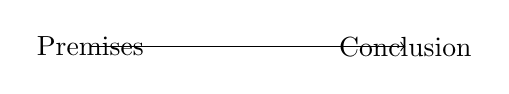
\begin{tikzpicture}[scale=.5]
      \node at (0,0) {Premises};
      \node at (8,0) {Conclusion};
      \draw[->] (0,0) -- (8,0);
    \end{tikzpicture}
    \caption{Propositional}
  \end{subfigure}
  \begin{subfigure}{.5\linewidth}
    \centering
    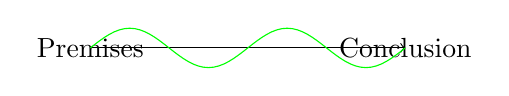
\begin{tikzpicture}[scale=.5]
      \node at (0,0) {Premises};
      \node at (8,0) {Conclusion};
      \draw[->] (0,0) -- (8,0);
      \draw[green] (0,0) sin (1,.5) cos (2,0) sin (3,-.5) cos (4,0) sin (5,.5) cos (6,0) sin (7,-.5) cos (8,0);
    \end{tikzpicture}
    \caption{Propositional and doxastic}
  \end{subfigure}
\end{figure}

\begin{note}[Propositional support]
  In the cases of interest, plausible that the agent `has' propositional support.
  For example, though in the type of scenarios the agent isn't provided direct information that they have some ability, the agent is provided with indirect information which hinges on some general ability.
  This general ability ensures epistemic reasons.
  In turn, sufficient epistemic reasons via potentive entailment.
\end{note}

\begin{note}[No doxastic support]
  A little more work to argue that the agent does not have doxastic support.
  Idea is to assume that agent forms attitude, and question whether it satisfies basing requirement.
  In part,~\ref{denied-claim}.
\end{note}


\begin{note}[Examining doxastic via basing]
  Following paragraphs serve two purposes.
  First, variety of accounts of basing are incompatible with doxastic support.
  Second, that the support in doxastic support is no different from support in propositional support --- relation to the agent.

  If already convinced, then may skip ahead.
\end{note}


\begin{note}[Taxonomy of basing]
  Follow taxonomy presented by \textcite{Korcz:2021ue}.
  \begin{itemize}
  \item Causal.
  \item Counterfactual.
  \item Doxastic.
  \item Causal-doxastic.
  \end{itemize}
\end{note}

\begin{note}[Causal]
  Causal is ruled out, as we're interested in support from general ability, roughly, and there's no plausible causal relation.
  The information that specific ability follows does the work.

  \cite{Moser:1989tv}
  \begin{quote}
    \emph{S}'s believing or assenting to \emph{P} is based on his justifying propositional reason \emph{Q} \(=_{\text{df}}\) \emph{S}'s believing or assenting to \emph{P} is causally sustained in a nondeviant manner by his believing or assenting to \emph{Q}, and by his associating \emph{P} and \emph{Q}.\nolinebreak
    \mbox{}\hfill\mbox{(\citeyear[157]{Moser:1989tv})}
  \end{quote}

  \begin{quote}
    \emph{S} occurrently satisfies an association relation between \emph{E} and \emph{P} \(=_{\text{df}}\)
    \begin{enumerate*}[label=(\roman*)]
    \item \emph{S} has a \emph{de re} awareness of \emph{E}'s supporting \emph{P}, and
    \item as a nondeviant result of this awareness, \emph{S} is in a dispositional state whereby if he were to focus his attention only on his evidence for \emph{P} (while all else remained the same), he would focus his attention on \emph{E}.
      \newline
      \mbox{}\hfill\mbox{(\citeyear[141--142]{Moser:1989tv})}
    \end{enumerate*}
  \end{quote}

  \cite{Ye:2020ux}
  \begin{quote}
    \textbf{Causation Caused by Believing (CCB)}

    One's belief that p is based on reason R just in case R causes the belief and the causation is caused by one's believing that R supports p.
    \newline
    \mbox{}\hfill\mbox{(\citeyear[27]{Ye:2020ux})}
  \end{quote}
  In our cases, no causation from premises.
  Further, if agent considers \ref{prem:ni}, then won't get the second part of supporting relation.
\end{note}

\begin{note}[Counterfactual]
  Counterfactual.
  Based on reason is caused or would have caused in appropriate circumstances.
  So, belief ends up being based on all pseudo-overdeterminants, for example.
  Built in to \citeauthor{Swain:1981wd}'s account is that the agent did some reasoning, and over-determinant is a substitute for reasoning performed.

  Here, may suggest that agent has done some reasoning, as they've gone from ability to conclusion.
  This reduces to an instance of \AR{} in order for agent to obtain support on reasoning \emph{performed}.
  No clear modification, as then agent would end up with a basic relation in cases where no relation obtains.
\end{note}


\begin{note}[Doxastic]
  Doxastic.
  \cite{Tolliver:1982us}

  \begin{quote}
    \begin{enumerate}[label=(B)]
    \item A bases his belief that q on p at time t, iff
      \begin{enumerate}[label=(\arabic*)]
      \item A believes that q at t and A believes that p at t, and
      \item A believes that the truth of p is evidence for the truth of q at t, and
      \item \space[\dots]\footnotemark\newline
        \mbox{}\hfill\mbox{(\citeyear[159]{Tolliver:1982us})}
      \end{enumerate}
    \end{enumerate}
    \footnotetext{
        The final condition is designed to rule out certain problematic cases which expands on \citeauthor{Tolliver:1982us}'s understanding of what it is for the truth of p to be evidence for the truth of q.
        \begin{quote}
        \begin{enumerate}[label=(\arabic*)]
          \setcounter{enumi}{2}
        \item Where A's estimate of the likelihood of q equals h at t \(0 < h \leq 1\), \emph{if it were the case that}:
          \begin{enumerate}[label=(\roman*)]
          \item A's second·order estimate ofthe L-proposition ``the likelihood of q is greater than or equal to h'' is less prior to t than it at t, and
          \item A did not believe p prior to t, and
          \item A came to belive pa at t,
          \end{enumerate}
          then, at t, A's second-order estimate of the L-proposition ``the likelihood of q is greater than or equal to h'' would be greater than it was prior to t.
          \end{enumerate}
        \end{quote}
      }
    The second condition qualifies \citeauthor{Tolliver:1982us}'s account as doxastic.
    The agent has a `meta-belief' that that the truth of the reason is evidence for the truth of the content of the agent's belief.
    For example, agent believes that the premises available for existence of (particular) strategy are evidence for existence of strategy.
    This does not require a causal relation between the reason and the belief, or between the relevant premises and the existence of the (particular) strategy.

    

    Feature of the meta-belief is that it is not part of the established basing relation.

    Two issues with \citeauthor{Tolliver:1982us}.
    A component of the first condition --- believing p at t --- and the second condition.

    On certain accounts of belief, believing p at t, will hold true.
    Whatever the relevant premises are, the agent believes them.
    However, this is not particularly clear.

    The second condition is the primary difficulty.
    Motivated by \citeauthor{Lehrer:1971aa}.
    \cite{Korcz:2000uo} outlines the argument (\citeyear[534]{Korcz:2000uo}).
    Hence, suggests such meta-beliefs are sometimes sufficient to establish basing relation.

    \citeauthor{Tolliver:1982us} talks of belief, \citeauthor{Korcz:2000uo} talks interchangeably of awareness or meta-belief.
    Continue to talk of meta-belief.

    \citeauthor{Tolliver:1982us} provides an analysis of what it is to believe that the truth of p is evidence for the truth of q. (\citeyear[156--157]{Tolliver:1982us})
    Key is that \citeauthor{Tolliver:1982us}'s condition requires the agent to have information about the relation.
    Incompatible with cases of interest, where agent doesn't have information about how (specific) ability leads to conclusion.

    \citeauthor{Korcz:2000uo} proposes that p and q contribute to causing the meta-belief.
    So, this suggests that the only cases are those in which there's some rewriting of an established basing relation.

    If follow \citeauthor{Korcz:2000uo}, then it seems as though we exclude instances of `first time' support.
    If we continue to follow \citeauthor{Tolliver:1982us}, then support for meta-belief.

    If don't require support, then things get difficult.
    On the one hand, problematic examples \citeauthor{Korcz:2000uo} mentions.
    As noted, \citeauthor{Korcz:2000uo} uses causation.
    Could substitute with some kind of support, but this kind of support is absent from scenarios of interest.

    On the other hand, if restricted independently of support, then it seems many basing instances are going to come for free.

    
  \end{quote}

  Here we have a kind of meta-belief about relation of support.
  As with counterfactual, the issue is with the meta-belief.
  No clear way to establish this without a variant of \AR{}.
  Here, this doesn't require~\ref{denied-claim}, which may be of some interest.

  Causal-doxastic inherit the problems of more basic.

  Upshot is that following the taxonomy, there's no clear basing relation in scenarios of interest.
  Influence of~\ref{denied-claim}.

  Of course, doesn't establish, as not requirement that doxastic support requires one such account of basing relation.
  However, more than suggestive that there's no doxastic support.

  In part, expected.
  Intuitively, agent is in distinct position from were they to establish doxastic support.
\end{note}

\begin{note}[Summarising]
  Seems plausible to grant that the agent has propositional support.
  Similarly plausible that the agent does not have doxastic support.

  Doxastic support captures something stronger than what is available to the agent.
  By doing reasoning, agent would establish doxastic support.

  Still, do not need to claim doxastic support.
  Goal is to allow agent to establish support from premises.
  This may fall (qualitatively) short of being doxastic support.

  Interest with above, as this is intuitively a case of, or closely related to, basing.
\end{note}

\begin{note}[First pass]
  Whatever it is that doxastic support and basing is, agent establishes this in potential event when witnessing.

  `Pre-basing'.

  Plausibility here is that propositional and doxastic support do not different with respect to support.
  Rather, differ with respect to relation between agent and support.
\end{note}

\begin{note}[Trace link in examples given]
  
\end{note}

\begin{note}[Example of \citeauthor{Neta:2019aa} on basing]
    \begin{quote}
    For an agent A to C for reason R involves A’s \emph{de se}, object-involving representation of a particular explanatory relation between R, on the one hand, and her C’ing, on the other, and that object-involving representation represents that same explanatory relation under the category ex post justifying.\nolinebreak
    \mbox{}\hfill\mbox{(\citeyear[204]{Neta:2019aa})}
  \end{quote}
  Distinct from other accounts.

  \emph{De se} so that there no possible mistake about whether it is the agent that is C'ing.
  The explanatory connexion is represented.
  \citeauthor{Neta:2019aa} is non-committal to what is involved with representation.

  Key is `\emph{that same explanatory relation}'.
\end{note}

\begin{note}[\future{}]
  Suggestion is to introduce idea of a \future{}.

  Understanding of doxastic support is appropriate connexion.
  Information about ability means that appropriate connexion may be established.
  A \future{} stands in place of the relation, it fixes that the attitude is connected to premises, etc.
  So, whatever the appropriate connexion would be, any resolution of the \future{} will satisfy that connexion, and the information about ability (in part) allows the agent to be confident that they may fulfil the \future{}.
\end{note}

\begin{note}[Intuition]
  At this point, a little intuition would be useful.
  Kind of like a \future{} from finance.
\end{note}

\begin{figure}[h!]
  \centering
  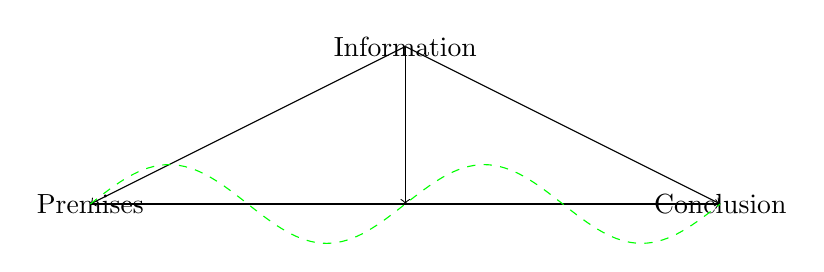
\begin{tikzpicture}
    \def\iHeight{2}
    \node at (4,\iHeight) {Information};
    \node at (0,0) {Premises};
    \node at (8,0) {Conclusion};
    \draw[->] (0,0) -- (8,0);
    \draw[->] (4,\iHeight) -- (8,0);
    \draw[->] (4,\iHeight) -- (0,0);
    \draw[->] (4,\iHeight) -- (4,0);
    \draw[green, dashed] (0,0) sin (1,.5) cos (2,0) sin (3,-.5) cos (4,0) sin (5,.5) cos (6,0) sin (7,-.5) cos (8,0);
  \end{tikzpicture}
  \caption{Sketch}
\end{figure}


\begin{note}[Expand tracking example]
  Consider tracking example.
  Here, on the relevant interpretation, the information provided to the novice allowed the novice to establish support relation.
  Understood here as providing information about to establish an appropriate connexion.
  And, given this information the novice goes ahead and establishes the (appropriate) connexion.

  Vary the example a little.
  Suppose the novice is provided with a book containing the information provided by the informer.
  Given understanding of base case, understand that the book is going to detail how to establish an appropriate connexion.
  Then, the novice reads the book, and fills in the detail.

  After reading the book, agent has doxastic support.

  Before reading the book, a more complex attitude.
  Conclusion on the basis of propositional support the novice has, and the result of establishing an (appropriate) connexion via the relevant contents of the book.
\end{note}

\begin{note}[New example]
  Consider an abbreviated proof.
  Look at the premises and conclusion.
  So, have propositional support.
  Quite tired, so fail to see how the conclusion is obtained from premises.

  On the one hand, this has been reviewed, etc.\ so route to doxastic support.
  However, given understanding of material, then after some sleep and a cup of coffee, you'll recreate the reasoning in detail.

  Hence, hold the conclusion on the basis of premises, with a \future{} representing the appropriate connexion to be filled in.

  
\end{note}

\begin{note}[Does not depend on application]
  The idea here is fairly general.
  Our interest is in support.
  However, it is more general.

  Simply tracing out something to be filled when required.
\end{note}

\begin{note}[Intuition, logic example]
  Final example by an analogy.

  Consider rules for existential.
  Take a fresh variable.
  Standard is to complete the proof by discharging the assumption.

  Instead, update the assignment function.

  So, three objects, some conditionals.
  Introduces some names.
  Not sure what the name refers to.
  Some property will be revealed, and interpretation fixed.
  
  Perhaps useful to think about in terms of existential reasoning.
  Here, however, we don't discharge the fresh variable.
  Rather, it hangs around in wait for fixed a reference via an updated assignment function.
\end{note}

\begin{note}[Deferring]
  So, \future{} is result of deferring establishing what the connexion is.
  At the time, the agent simply establishes the connexion on the basis of the information they have.
\end{note}

\begin{note}[Existential]
  Support is flowing from the premises to the conclusion.
  It is not from ability.

  Difference is clearest when considering the instance of \AR{} in which the agent appealed to the attribute of having propositional support for the conclusion.
  In the case of \AR{} the agent did not appeal to the propositional support.
  Rather, the agent appealed to having propositional support.

  Contrast, \WR{} takes the propositional support that satisfies the existential.
\end{note}

\begin{note}[Contrast with \ref{denied-claim}]
  Noted that \ref{denied-claim} is understood with respect to doxastic, and here's where the incompatibility comes in.
  For, \ref{denied-claim} holds that a \future{} is no good.
\end{note}

\begin{note}[Asynchronous]
  Asynchronous, as reasoning is deferred.
  Some difficulty.
  However, `weak' asynchronous, as the support `exists', so to speak.
\end{note}

\begin{note}[Key difference]
  The key difference between \AR{} and \WR{} is that with \WR{} the agent does not rely on ability/potential event for support.
  Rather, the agent relies on the support that they have for the premises which is independent of the ability information.

  Information in \WR{} does not support conclusion.
\end{note}

\begin{note}[Another difficulty]
  Another difficulty with the first pass is tight connexion with propositional support.
  Increase in information, etc.
  Seems as though the agent may obtain conclusion of distinct propositional support.

  Chess example, there may be multiple strategies.
  One is sufficient.

  Other examples are more complex.
  For example, proof.
  Study, develop understanding of domain.
  Additional premises available.
  Does this resolve the \future{}?

  Perhaps not, agent no longer has a need to resolve the particular \future{}.

  However, as in the case of multiple strategies, plausible that additional premises fold into the same \future{}.
  So long as there remains a potential witnessing event, it seems any witness should resolve the \future{}.

  Some improvements may be made.
  First, detail a more pressing difficulty.
\end{note}

\subsubsection{Difficulty with first pass}
\label{sec:diff-with-first}

\begin{note}[Overview]
  The first pass assumed something about propositional support.
  That there is propositional support whether or not the agent does the reasoning.

  Whether or not agree with assumption, consider a pair of contrasting accounts of propositional support, and see how this assumption is important.

  After so doing, consider whether we can avoid assumption made.
\end{note}

\begin{note}[Different view of propositional]
  For example, \citeauthor{Turri:2010aa} argues for~\ref{Turri:PJ}.
  \begin{quote}
    \begin{enumerate}[label=(\textbf{PJ}), ref=(\textbf{PJ})]
    \item\label{Turri:PJ} Necessarily, for all \emph{S}, \emph{p}, and \emph{t}, if \emph{p} is propositionally justified for \emph{S} at \emph{t}, then p\emph{} is propositionally justified for \emph{S} at \emph{t} \textsc{because} \emph{S} currently possesses at least one means of coming to believe \emph{p} such that, were \emph{S} to believe \emph{p} in one of those ways, \emph{S}'s belief would thereby be doxastically justified.
    \end{enumerate}
  \end{quote}
  If so, then the availability of propositional support is secured by the potential event of reasoning.
  Hence, it seems that this reduces to a case of \AR{}.
  For, if the agent does not appeal to support for witnessing event, then the agent does not have grounds for holding that they have support for conclusion.
  It is not sufficient to observe that the agent has support so long as information about potential holds.
  Instead, the potential is doing the work in providing the agent with propositional support.

  Of course, \citeauthor{Turri:2010aa} doesn't require that the agent be aware.
  But this doesn't solve the problem.
  The issue is that the two instances of support coincide.

  It's somewhat straightforward to recast (\emph{PJ}) as `because the agent has the ability'.
  Indeed, \citeauthor{Turri:2010aa} speculates that propositional support is governed by abilities.
  Though, the exact relation between \citeauthor{Turri:2010aa}'s constraints and are use of ability is unclear.
  At the very least, \citeauthor{Turri:2010aa}'s seems weaker, as we require a sufficient collection of preconditions to be satisfied.
\end{note}

\begin{note}[Note]
  The difficulty is that if \citeauthor{Turri:2010aa} is followed, then there's no support to do the work.
  This does not mean that the premises are unavailable.
  Instead, the premises are inert.
\end{note}

\begin{note}[Same from \citeauthor{Goldman:1979ui}]
  \citeauthor{Goldman:1979ui} proposes \emph{ex ante} justification.
  \begin{quote}
    Person \emph{S} is \emph{ex ante} justified in believing \emph{p} at \emph{t} if and only if there is a reliable beliefforming operation available to S which is such that if \emph{S} applied that operation to his total cognitive state at \emph{t}, \emph{S} would believe \emph{p} at \emph{t}-plus-delta (for a suitably small delta) and that belief would be \emph{ex post} justified.\nolinebreak
    \mbox{}\hfill\mbox{(\citeauthor[21]{Goldman:1979ui})}
  \end{quote}
  Note that \citeauthor{Goldman:1979ui} talks of the `total cognitive state' of the agent at \emph{t}-plus-delta.
  It seems clear that the cognitive state of the agent at \emph{t} is relevant on in so far as the delta in \emph{t}-plus-delta is suitably small.
\end{note}

\begin{note}[Example?]
  However, following present line of thought, propositional support is a derived relation.
  It is a relation derived from some `attribute'.

  Clearest to see by recalling reasoning above.
  Project from event.
\end{note}

\begin{note}[Basic point]
  The observation here is that these accounts may taken as trouble for \WR{}, and in turn as partial support for \AR{}.
  Partial support for \AR{} as these accounts of propositional support are of propositional rather than doxastic support, and \AR{} is concerned with doxastic support.
  So, need to be furnished to show that an agent has the option of obtaining support for the conclusion of the reasoning that they are able to perform.

  It seems rather that this is an objection to the basic idea of \WR{}.
\end{note}

\begin{note}[This is trouble from \WR{}/Something about evidential relations]
  Not that these come easy.

  Basic understanding of propositional support.
  Seems support is a relation between premises and conclusion, or base and proposition.

  Common to talk in terms of `\emph{p} is propositional justified for \emph{S}'.
  Here, though, expanded.
  Sufficient reasons to believe that \emph{p}, and \emph{S} has those reasons.

  And, \textcite{Silva:2020aa} highlights troubles with evidential relations, and epistemic reasons.

  Similarly, because \emph{S} has ability, \emph{S} ought not to hold that \dots
\end{note}

\begin{note}[Bracketing possible issue]
  A possible lesson to be drawn from \citeauthor{Turri:2010aa} and \citeauthor{Goldman:1979ui} is that there is no clear relation of support between premises and conclusion.
  Don't make sense to subdivide the agent's total cognitive state, or separate the means by which the agent may come to believe \emph{p}.

  This is the foundation of a challenge to~\ref{prem:bP}.

  However, this isn't too much of a concern.
  Important for our purposes is preconditions.
  Talk of premises, is intuitive, what we're after, though, is some way of obtaining support which doesn't reduce to \AR{}.
\end{note}

\subsubsection{Second pass: \future{} support}
\label{sec:second-pass:-futures}

\begin{note}[Is this only surface deep?]
  Introduced the idea of a \future{}.
  Allowed an agent to establish doxastic support on basis of `pre-existing' propositional support.

  The primary problem with the first pass in terms of propositional support stems from the possibilities of reducing propositional support to doxastic support.
  Hence, if reduction, then the understanding of \WR{} in terms of propositional support reduces to an instance of \AR{} --- support for premises that the agent appeals to just is the support the agent has for ability, or potential event in which agent witness the relevant action.

  Due to role of propositional support, then, any variation on the basic idea will inherit this issue.
  Tentatively, then, \WR{} requires a particular understanding of propositional support.

  Note, this is only a problem for one part of the first pass.
  Do not have the option of relying on pre-existing support relation.

  That the premises must stand in an existing support relation may be challenged.

  We have already seen that it is plausible that any support obtained prior to witnessing the reasoning is distinct from the support that would be obtain by witnessing the reasoning.

  Suggestion is that support flows through `\future{}' relation of support.
  Avoids propositional support.
  Additional benefits.
\end{note}

\begin{note}[Support]
  Well, the point here is that the support relation may be considered with an reference that has not yet been fixed.

  So, instead of taking a `pre-existing' support relation, as in the case of propositional support, obtain support because the support established in potential event may be `brought forward' by establishing premises and relation whose referent is `deferred'.

  The novelty here is that support transmits through `deferred' support.
\end{note}

\begin{note}[Asynchronous]
  Intuitively, this is asynchronous.
  The agent establishes relation of support given information.
  Then, at some other times details exactly what the relation of support is.
  The unique thing in these cases is that the agent has information about what the result of the deferred detailing is, and thus has the option of establishing a relation of support to be filled in.

  Always in terms of potential witnessing event.
  Information the agent has grants witnessing event.
  Preserved under variation of premises, so long as potential event remains.

  Contrast to propositional support, which did not require anything asynchronous.
\end{note}

\begin{note}[Promises]
  Introduced in \textcite{Liskov:1988vo}.
  Decouple process of establishing relation support, and detailed what the relation of support is.

  Information that the agent has the ability, or that there is a potential event, is used to create a promise.
  However, support is distinct from this.
\end{note}

\begin{note}[The really important thing]
  Support is flowing from the premises to the conclusion.
  It is not from ability.

  If propositional support that does not reduce to ability, then no need to take this as a primitive.
  If not, then perhaps.
\end{note}

\begin{note}[Why does the agent obtain support?]
  A \future{} is something of a primitive.
  And support is very general.
  So, not really possible to work from some more basic premises.

  Instead, consider it a hybrid of the two types of propositional support considered.
  Like general propositional support, holds whether or not agent has done reasoning.
  Like \citeauthor{Goldman:1979ui} etc.\ potential events inform.

  Not assuming propositional support.
  Or, assuming that information about potential event may not provide information about pre-existing relation of support.
  So, where does support come from?

  Well, we've got a \future{}.
  Associated promise.
  The promise is not providing support.

  What is added is specification of how agent obtains support for conclusion.

  The potential event, then, ensures that support may be obtained.

  Support for conclusion because potential event provides sufficient information guarantee relation of support may be established.
  What remains is fixing the specifics.

  The support for the conclusion just is the support that the agent would obtain from witnessing.
  The thing is that the reasoning part is the only thing that's missing.
  It's the details that are deferred.
  I.e.\ asynchronous.

  Illustration with standard case, then cutting a pasting for a different temporal order.
\end{note}

\begin{note}[Social parallels]
  Relationship between inter-personal and intra-personal agency.

  Difficulty with inter-personal as testimony.
  However, have noted from \citeauthor{Easwaran:2009tm} that certain cases information about entailment and support come apart.

  This relates to `buck-passing' (\citeyear{Baker:2018aa})
  \textcite{Baker:2018aa} suggest `strong buck-passing'

  \begin{quote}
    \textbf{Strong B-P:} When challenged to produce the evidence that justifies her belief that p, A can acknowledge that she is unable to do so by herself, without help from her source, without thereby undermining her claim to know that p.\nolinebreak
    \mbox{}\hfill\mbox{(\citeyear[8]{Baker:2018aa})}
  \end{quote}
  \citeauthor{Baker:2018aa} don't directly argue for strong buck-passing.
  Instead, suggest that it has certain advantages given independent commitments regarding testimony.

  Kind of considerations that motivate \citeauthor{Easwaran:2009tm}'s view on transferability suggest plausibility of buck-passing.
  Place as intermediary between two skilled mathematicians.
  Intermediary will pass the buck to presenter when questioned by agent.
  For, proof is transferable.
  And, intuitively does so because testimony is not required.

  The agent then doesn't seem to be in the same position.
\end{note}

\begin{note}[Other cases]
  Thinking back to the tracking case may be helpful.
  In the case, information allowed the agent to establish (doxastic) relation of support.

  If propositional support doesn't work as expected, then prior the agent did not have propositional support.
  (This is a plausible reading of \citeauthor{Turri:2010aa}'s remarks on the more fundamental stuff that goes on with support, though could be avoided.)

  The difference is that the information is restricted in the case of interest.
  But the \future{} \emph{functions} in an analogous way.
  It just doesn't carry (sufficient) information about the relation.
\end{note}


\begin{note}[How support works]
  In the case of reasoning, the result will be that the agent has information about premises.
  Here, it is important to note that the agent has `propositional' support for the premises, independent of the ability information.
  So, the agent does not need to appeal to the existence of the event as a premise in obtaining support for the conclusion.
  The only relevant support the agent has is the support for the premises.
\end{note}

\begin{note}[Similar applications of the basic idea]
  Introduce idea that this is something of a placeholder.
  Perhaps use the example from names with an as yet unidentified reference to provide additional motivation.

  The idea is similar in principle.
  There is someone out there in the world.
  Just as there is support that the agent may use.
  So, the remaining task is to fix the interpretation of the name.
  Likewise, the remaining task for the agent is to witness the relation of support.

  In both cases, establishing the additional stuff is useful.
  Foremost, resolves the possibility that the `\future{}' may not be resolved.
  And, other minor benefits in terms of further information.
\end{note}

\begin{note}[Giving up on synchronous support]
  This is something of a cost.
  Cost captured in large part by~\ref{denied-claim}.

  Difficult.
  For, if basic understanding of propositional support, then still require something to explain how the agent transforms this to doxastic support.

  Still, two plausible pictures.
  Pre-existing propositional support.
  Support obtained through use of a \future{}.
\end{note}

\begin{note}[Upshot]
  Main upshot is relation of support.

  One nice upshot is that there is a clear link between the support obtained prior to reasoning, and the support obtained by reasoning.
  It's filling in the deferred reasoning.

  May expand.
  For example, with a promise to resolve the support relation.

  Another upshot is that ???
\end{note}


\subsection{Distinction between \AR{} and \WR{}}
\label{sec:dist-betw-ar}

\begin{note}[Overview]
  The important difference is what supports the conclusion.

  Here, we suggest that further differences depend on additional commitments.
\end{note}


\begin{note}[Key Issue]
  The key issue is whether the agent obtains support for all the relevant preconditions of witnessing the ability by witnessing.
  And, whatever follows from this, e.g.\ in terms of commitments and so on.

  If so, then anything that follows from \AR{} also follows from \WR{}.
  Conversely, as the agent does not obtain information about how the ability is witnessed, it seems what follows from \WR{} also follows from \AR{}.
\end{note}

\begin{note}[Interesting case]
  Interesting case to think about, in which the agent obtains support for what follows from witnessing, but intuitively not for some other precondition.
  \begin{itemize}
  \item Ability to reason to \(\phi\).
  \end{itemize}
  Entailment applies to \(\phi\).
  Entailment doesn't seem to apply to reasoning to \(\lnot\phi\) as mistaken.
\end{note}

Understanding of ability is such that there is always a potential witnessing event.

\ref{denied-claim} and~\ref{prem:ni} are universal claims.
\ref{prem:ab} is an existential claim.
\ref{denied-claim} and~\ref{prem:ni} clash in scenarios where the possibility captured in~\ref{prem:ab} is realised.

The collection of~\ref{denied-claim},~\ref{prem:ni}, and~\ref{prem:ab} is in tension.

There is an additional secondary premise:

\begin{note}[Two ways to understand ability and support]
\begin{enumerate}
\item\label{prem:ability} Two ways to obtain conclusion given ability.
  \begin{enumerate}
  \item Attribution.
  \item Witnessing.
  \end{enumerate}
\end{enumerate}

\ref{prem:ability} does not make a claim about any particular use of ability.
As a template, conceptually (or logically) coherent.
If there's a problem, then it's because there are further constraints on understanding of support.
\end{note}

\section{Miscellaneous}
\label{sec:misc}

\subsection{\citeauthor{Audi:1983ux} on \citeauthor{Lehrer:1971aa}}
\label{sec:lehrer}

\begin{note}[Lehrer]
  \citeauthor{Lehrer:1971aa}'s cases are somewhat of interest.

  Here, we have an agent who seems to have both propositional some proposition.
  The propositional support is stipulated as unquestionably good, take this to be established however one likes.
  However, obtaining doxastic support is difficult, and the agent does not recognise that they have propositional support.
  Instead, the agent forms a contrary attitude based on contrary propositional support.

  So we have:
  \begin{enumerate}
  \item\label{L:gl:prop:p} Propositional support for \(\phi\)
  \item\label{L:gl:prop:not-p} Propositional support for \(\lnot\phi\)
  \end{enumerate}
  Were the support for \(\phi\) is stronger than the support for \(\lnot\phi\).
  And, the haven't has established doxastic support for \(\lnot\phi\).
  As the agent has not established doxastic support for \(\phi\) (due to difficulty), the agent believes \(\lnot\phi\).

  The agent then is then informed by some source that the agent has (stronger) propositional support for \(\phi\).
  The agent then goes and establishes doxastic support for \(\phi\).
  However, due to the complexities involved, the agent is not swayed by the doxastic support.
  For example, some errors.
  However, because the source provided information that propositional support is stronger, agent revises attitude in favour of \(\phi\).
\end{note}

\begin{note}[Example]
  \citeauthor{Lehrer:1971aa} specific example involves a questionable source, and it is unclear whether there's much to be said for the agent.

  Variant with student.
  Student attempts to prove something.
  It's quite difficult, and the agent's intuitive understanding of the domain guides them to \(\lnot\phi\).
  So, student has strong belief that \(\lnot\phi\) is the case, though lacks knowledge --- the student has not ruled out that \(\phi\) is the case.
  Teacher suggests that the material establishes \(\phi\).
  Student takes a second look, and following the formalism, proves that \(\phi\).
  However, the agent has no intuitive understanding (some of the) key steps in the proof.
  So, the agent relies on the teacher.
\end{note}

\begin{note}[Possible to read \citeauthor{Lehrer:1971aa}'s example as similar]
  If the agent obtains support for \(\phi\), then it seems this is due to the propositional support the agent has, rather than the doxastic support that the agent forms.
\end{note}

\begin{note}[\textcite{Audi:1983ux}]
  \citeauthor{Audi:1983ux} presents a neat summary of how the argument may go:
  \begin{quote}
    Since
    \begin{enumerate*}[label=(\arabic*)]
    \item\label{Audi:divergence:1} the justification of the belief that \emph{p} is \emph{q}, which is good evidence for \emph{p}, and
    \item\label{Audi:divergence:2} S believes \emph{q}, and sees its full evidential bearing on \emph{p},
    \item\label{Audi:divergence:3} S has good evidence for \emph{p}.
      Hence,
    \item\label{Audi:divergence:4} S has a justification for the belief that \emph{p}.
      Thus,
    \item\label{Audi:divergence:5} if S believes \emph{p}, then even if his believing \emph{p} is not to any degree sustained by his believing \emph{q}, he justifiably believes \emph{p}, and the (or a) justification of this belief is based on his belief that \emph{q}.
    \end{enumerate*}
    \nolinebreak
    \mbox{}\hfill\mbox{(\citeauthor[406]{Audi:1983ux})}
  \end{quote}
  \citeauthor{Audi:1983ux} suggests the argument falters from step~\ref{Audi:divergence:4} to~\ref{Audi:divergence:5}.
  In short, the agent doesn't get doxastic support from proposition support.
\end{note}

\begin{note}[Important difference]
  There is an important difference between the two types of cases.
  In the \citeauthor{Lehrer:1971aa} type cases, the agent discards the doxastic support.
  In our type of case, the agent has not yet obtained doxastic support (implicit has been that the agent would obtain doxastic support).

  So, in our cases, there is scope to reject~\ref{Audi:divergence:5}.
  Do need some kind of sustaining, and the use of information about ability establishes the relevant sustaining.
\end{note}

\begin{note}[Notes for the moment]
  Todo is to work through \citeauthor{Audi:1983ux} in some detail and see if there's a stronger argument against the position I endorse.

  A potentially important point is that there's no counterfactual dependency in \citeauthor{Lehrer:1971aa}'s cases, while there is some kind of counterfactual dependency in the cases of interest.

  Should check: \textcite{Tierney:2012tt}.
\end{note}


\subsection{Additional observations}
\label{sec:addit-observ}

\begin{note}[Trouble with modals]
  We have sketched potentive entailment.
  However, noting the interaction between a modal and a verb.

  Understanding of why the entailment works has been left largely to intuition.

  The specifics of potentive entailment are not too important, so we may omit the detour.
  Still, even for those willing to make the detour it is not clear how long it would take, or where it would lead.

  Difficulty is seen by taking a straightforward treatment of the modals involved.

  `There is potential for' and `agent S has the (specific) ability to' are modals.

  Standard first pass at modals, via possible worlds and accessibility relations.

  Before continuing further, the presence of difficulty may be quickly noted by noting the similarities between potentive and actuality entailments.
  \textcite{Alxatib:2019wf} provides the following account of actuality entailments.
  \begin{quote}
    Actuality Entailments (AEs) are inferences from premises that appear to be modal, like (1a), but their content is that the modality is effectuated in the evaluation world --- (1b).

    \begin{enumerate}[label=(\arabic*)]
    \item
      \begin{enumerate}[label=\alph*.]
      \item Pierre a dû \hspace{26pt} prendre le \hspace{3.5pt} train \newline
        Pierre had.to.\textsc{pfv} take \hspace{14pt} the train\newline
        \hspace{-4pt} ‘Pierre had to take the train'
      \item \emph{Inference}: Pierre took the train.\nolinebreak
    \mbox{}\hfill\mbox{(\citeyear[701]{Alxatib:2019wf})}
      \end{enumerate}
    \end{enumerate}
  \end{quote}

  Note, the reading of `had' in (1a) is `unambiguously deontic' (\citeyear[703]{Alxatib:2019wf}).
  English paraphrase does not carry the same entailment, but does seem to carry a corresponding implicature.

  Potentive entailment is related, but it is not (necessarily) the \emph{content} on the modality that is effectuated in the evaluation world (though it may be).
  Following the account of actuality entailments, \citeauthor{Alxatib:2019wf} highlights the basic problem:

  \begin{quote}
    AEs are surprising; if we assume that modals attribute their propositional argument to potentially non-actual worlds, something must be special to AE-licensers that leads to the inference of actuality.

    Whatever that special feature is, its effect is complex, and it interacts in nontrivial ways with other phenomena of theoretical interest.\nolinebreak
    \mbox{}\hfill\mbox{(\citeyear[701]{Alxatib:2019wf})}
  \end{quote}

  Possible world, then the event takes place in the possible world.
  Had takes some ordering, so best world involved taking the train.
  This doesn't seem to explain why Pierre took the train.

  Similar with potentive.
  There is a possible world, but it's not obvious why this constrains the world of evaluation.

  With examples, it is clear that there is an entailment.
  Substituting different verbs and results, entailment goes away.

  This isn't too helpful.
  For, we would see what is required to be the case at the possible world.
  However, the consequent of a potentive entailment holds at the world of evaluation.

  Of the form \(\Diamond \phi \rightarrow \psi\).
  So, \(\lnot \psi \rightarrow \Box \lnot \phi\).

  Potential clue.
  Restrictor.
  In effect, the potentive entailment is drawing out information about the restrictor/modal base.

  Figuring out the relevant construction of modal base \dots well \dots
  Something of a dead end.
\end{note}

\begin{note}[More on actuality entailment]
  The potentive entailment is not an actuality entailment.

  \begin{quote}
    \begin{enumerate}
    \item Yesterday, John was able to eat five apples in an hour. (past episodic)
    \item In those days, John was able to eat five apples in an hour. (past generic)
    \end{enumerate}
    (315a) implicates that John actually ate five apples in an hour.\nolinebreak
    \mbox{}\hfill\mbox{(\citeyear[173]{Bhatt:2008aa})}
  \end{quote}

  \begin{quote}
    (317) Last night, a masked assailant attacked me on my way home.
    I was able to wrestle him to the ground.
    \#But I didn't do anything since I am a pacifist.\nolinebreak
    \mbox{}\hfill\mbox{(\citeyear[174]{Bhatt:2008aa})}
  \end{quote}

  Key here is the entailment is restricted to the event, and the modal needs to be in the past tense.
  (\textcite{Pinon:2003te} has some nice examples.)
  Of course, potentive entailment applies.
  Certain conditions had to be in place in order for there to have been a witness of ability.
  Still, these seem to be distinct as they do not conform to the same restriction placed on actuality entailment.

  There is some work on the difficulties involved in obtaining the actuality entailment.
  \citeauthor{Bhatt:2008aa,Bhatt:1999ud} argues that the entailment doesn't follow from ability attribution.
\end{note}


\subsection{Agentive modals}
\label{sec:agentive-modals}

\begin{note}[Summary]
  This is something of an appendix to the present chapter.
  The goal is to review the literature on agentive modals, and highlight that there is some difficulty with obtaining a clear understanding of potentive entailment from the proposals made.
\end{note}

\begin{note}[Agentive modals]
  Agent is able to \dots

  Ability modal.

  \begin{enumerate}
  \item It is possible that Y stole the jewels.
  \item S has the ability to prove that Y stole the jewels.
  \end{enumerate}

  The ability statements of interest are an instance of agentive modality.
  \cite{Mandelkern:2017aa}
  \cite{Maier:2013vk}
  \cite{Schwarz:2020aa}
  \cite{Willer:2021ur}
  \cite{Maier:2021te}

  Some proposals, and some issues.
  E.g.\ Kratzer on `can'.
  The dart board problem.

  For the moment, leave the literature on ability modals aside.
  Focus is on specific ability.
  And, in particular, ability to reason.
  Literature focuses on non-mental actions.
  Throwing darts, unlocking safes, etc.
  In most cases the result of witnessing the ability depends on witnessing the ability.
  If the agent does not throw the dart, it will not land on the board.
  If the agent does not unlock the safe, then the safe will not be unlocked.

  Some further details in section~\ref{sec:agentive-modals}
\end{note}

\begin{note}[No volition]
  Tempting to restate in terms of volition.
  For example, paper.
  Presents some difficulty, especially given the observation that the agent may not at present have the volition.
  For, then to evaluate the entailment, need to consider some counterfactual possibility.

  S is able to prove that Y stole the jewels.

  This is because S is heavily involved.
  S has no volition to do so.
  This would result in estrangement for S.
  Without some complexity, it seems that in order to assume S has the volition, we would need to assume that S was not involved.
  Therefore, in turn, that the jewels were not stolen, or that the resulting proof would be different from what it actually is.
\end{note}

\begin{note}[Potentive entailment and modals]
  Given sufficient context, instances of the potentive entailment apply.
  There are darts available, there is a safe.

  Further, focusing on the modal aspect leads us to some difficulties.
  The entailment tells us about how things are in order for something to be possible.
  It is not clear how to conceptualise this.
  Consider possibility.
  In general, no potentive entailment.
  It is possible that the sun rises from the west.
  Unclear what follows about how things actually are from this.

  Properties of the accessibility relation?
\end{note}

\begin{note}[???]
  Doesn't rule out property.
  Don't get into the ontology of potential events.
  So, may reduce.
  Still, from the perspective of reasoning, not required.
  Entailment follows from potential, and potential may require attribution of ability, but only from some ontological perspective.
\end{note}


\section{Formal?}
\label{sec:formal}

\subsubsection{Obtaining potentive entailments}
\label{sec:obta-potent-enta}

\begin{note}[Quick sketch]
  This is an optional section.
  We explained potentive entailment and given examples.

  Reader may wish for a technical account.
  In this section we sketch one such account.

  We do not argue that the account is wholly adequate.
  However, functional at first pass.

  Two things to do.
  \begin{enumerate}
  \item Establish some equivalence between potential and ability.
  \item Given an account of the potentive entailment.
  \end{enumerate}

  Start by taking a simple possibility understanding of the modal and show how potential and ability fit.
  We will then build on the possibility understanding to fix potentive entailment.
\end{note}

\subsubsection{Modal}
\label{sec:modal}

\begin{note}[Potentive]
  The potentive is straightforward to analyse.

  Fairly clear understanding of event semantics.

  Here, existential quantification over events is replaced by a modal.

  This requires some non-standard existential, but we're not too interested in providing an analysis suitable for semantics.
\end{note}

\begin{note}[Ability]
  Our understanding of ability is basically the same as potentive.

  Ability functions as an equivalent quantifier.
\end{note}

\begin{note}[Avoid ability?]
  A simple corollary of the above observations potentive entailment does not require ability.

  If it is possible to provide information about potential event of reasoning without attributing ability, then we don't need to speak of ability at all, perhaps with the exception of generating intuitive scenarios.

  May wonder how important ability is.

  Difficult case.
  Go for externalism, and co-reference.
  State a conclusion, but the agent would not reason to the conclusion under that description.

  There's a potential event, but it isn't clear that the agent has the ability.

  Doubt this is possible, as agent needs to do something.
  And, ability this seems sufficient for an ability statement.
  So, continue to work with ability.
\end{note}

\begin{note}[Some formal stuff]
  \[(\text{Able}(s,e) \land (V(e) \land \text{agent} = s \land \text{result}(e) = \phi))\]
  There is some event \(e\), such that \emph{s} is able to bring about, and \(e\) consists of \emph{s} \emph{V}ing with the result that \(\phi\).

  The quantification here is somewhat familiar to Lewis' counterpart theory.

  Understand ability as relating the agent directly to an event.
  Alternative it to take a truth value.
  \((\text{Able}(s,\exists (V(e) \land \text{agent} = s \land \text{result}(e) = \phi))\).

  Close to having a possible world with \(\phi\) and accessibility relation.
  Interpret the non-standard existential in this way, if it helps.
  There is some possible world and some event in that world, such that the agent at the world of evaluation is able to perform the event witnessed at the possible world.

  In both cases, it's the role of the event.

  \begin{figure}[h]
    \begin{subfigure}{.5\textwidth}
      \centering
      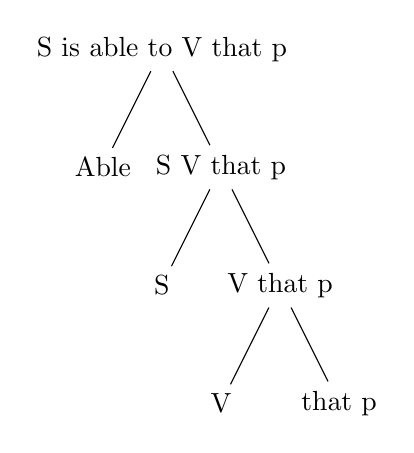
\begin{tikzpicture}[
        ]
        \node{S is able to V that p}
        child {node {Able}}
        child {node {S V that p}
          child {node {S}}
          child {node {V that p}
            child {node {V}
            }
            child {node {that p}
            }
          }
        };
      \end{tikzpicture}
    \end{subfigure}
    %
    \begin{subfigure}{.5\textwidth}
      \centering
      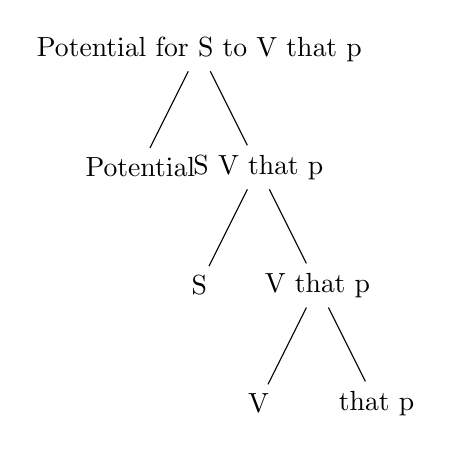
\begin{tikzpicture}[
        ]
        \node{Potential for S to V that p}
        child {node {Potential}}
        child {node {S V that p}
          child {node {S}}
          child {node {V that p}
            child {node {V}
            }
            child {node {that p}
            }
          }
        };
      \end{tikzpicture}
    \end{subfigure}
  \end{figure}
  Suggestion here is that there's really nothing too interesting.
  In both cases it seems possible to have a complete description of the witnessing event prior to the introduction of a modal.
  Only complexity involved is projecting agent from event in order to apply ability.
\end{note}


\begin{note}[Breaking things down]
  An instance of potentive entailment has an antecedent and consequent.
  As may be seen from the examples provided, there are no particular constraints on the consequent of a potentive entailment.
  The antecedent of potentive entailments of interest, however, have two main components:
  \begin{itemize}
  \item\label{pe:part:event} An event.
  \item\label{pe:part:modal} A `potentive' modal applied to the event
  \end{itemize}
  The event in turn has three important components:
  \begin{enumerate}
  \item\label{pe:part:agent} An agent.
  \item\label{pe:part:verb} A verb describing some action performed by the agent.
  \item\label{pe:part:result} Some result of a successful performance of the action described by the verb.
  \end{enumerate}

  Gave a gloss of potentive entailment.

  Key observation 1.
  Possible consequents are determined by the event, rather than the modal.
  Obtain consequent because of the modal.

  So, each of the examples, we obtain the same entailment on the assumption that the event described has happened.

  Contrast.
  Potential for \(e_{1}\) and potential for \(e_{2}\), so potential for \(e_{3}\).
  E.g.\ conjunction introduction.

  In other words, the consequent does not hold because the event is a \emph{potential} event.
  Or, that this is `epistemic'.

  Well, consequent because the event of the antecedent requires the consequent.

  So, that the potential provides a way to get the consequent prior to the event happening.
  No instance of potentive entailment where the consequent follows because the event is potential.
  This is not to deny that there are cases in which entailment relies on potential.

  So, here explaining why the work is done primarily by the verb.
  Might think that using `discovers' is a counterexample.
  Only possible because the action involved is for the moment potential.
  However, the verb itself does the work here.
  Get the consequent that the agent hasn't done the reasoning, but understanding this as simply shifting temporal index.

  So, the important of this key observation is that we further reduce interest in ability.
  We've seen that alternative modal may be used.
  And now that the modal is of secondary importance.

  So, property is seen as surface level.

  Two candidates for the antecedent.
  \begin{quote}
    \begin{enumerate}
    \item There is a potential event in which \emph{S} \emph{V}s that \(\phi\).
    \item \emph{S} has the ability to \emph{V} that \(\phi\).
    \end{enumerate}
  \end{quote}
\end{note}


\subsubsection{Entailment}
\label{sec:entailment-1}




\begin{note}[Counterfactual]
  One option is counterfactual.
  This is true, and then consider all of those things some that if they we're true, potential wouldn't be true.
  Consider change to the actual world that would result from false consequent, and figure out whether potential still holds.

  Problem here is that counterfactuals are tricky.

  Minimal change may still result in potential.
  Chess example, if strategy doesn't exist, then it's not clear how to understand this.
  Some other rules of chess, and strategy may still exist.
\end{note}

\begin{note}[More direct]
  Preferred option is to consider all witnessing events.
  No matter how things turn out, the truth of \(\phi\) persists throughout event.

  What about changes?
  So, there's some potential event, because of some change to the rules of chess.
  Hence, there is a possible event, but relies on an unexpected development.
  Problem with potential?
  Arguably same issue holds for ability.

  However, it's then going to be the case that there is some change.
  Problem here when it comes to reasons, as the agent doesn't have the reasons available.

  Observation here is that \(\phi\) is an enabling condition.
  Potential just in case that it does not depend on further enabling conditions that are not yet the case.


  So, suggestion that if something holds throughout every event, then it holds of the actual world.
  Basically, this rules out an enabling condition that is not true.

  Hence, \(\phi\) is an enabling condition, and does not require additional enabling conditions.
\end{note}

\begin{note}[Still issue of underspecified event]
  Returning to the matchbox.
  Different preconditions.
  Well, depends on how the event is understood.

  Use this idea to suggest some troubles.
  By, extending events to include establishing what seem to be preconditions.
  Suggest that this is taken care of by understanding of event.
\end{note}

\begin{note}[Some issues with ability]
  Even so, not clear that additional features of ability are desirable.
  For example, conditional analysis.
  S has the ability to \(\phi\), understood as S would \(\phi\) if S tried to.
  (\citeyear[\S4]{Mandelkern:2017aa})
  And act conditional analysis
  \begin{quote}
    there is some practically available action A such that the closest world where S tries to do A is a world where S does \(\phi\)\nolinebreak
    \mbox{}\hfill\mbox{(\citeyear[\S5]{Mandelkern:2017aa})}
  \end{quote}
  Or \cite{Schwarz:2020aa}, who distinguishes two readings.
  \begin{quote}
    \begin{enumerate}[label=\textbf{\alph*.}]
    \item \emph{S} can \(\phi\) (effectively) iff there are (highest-ranked) accessible worlds at which \emph{S} \(\phi\)s.
    \item \emph{S} can \(\phi\) (transparently) iff there are (highest-ranked) accessible worlds at which \emph{S} \(\phi\)s \emph{transparently}.
    \end{enumerate}
    \emph{S} \(\phi\)s \emph{transparently} iff \emph{S} \(\phi\)s as a result of a volitional state that warrants believing that she will \(\phi\) provided that \(\phi\)ing is under her volitional control.
  \end{quote}

  \begin{quote}
    a world is accessible iff it is under the agent’s volitional control --- that is, iff it would result from some available variation of the agent's volitional state.\nolinebreak
    \mbox{}\hfill\mbox{(\citeyear{Schwarz:2020aa})}
  \end{quote}

  Accessible world in which agent has volition.

  
  Counterfactual considerations.
  



  Noted that potential events don't require agents, hence if volitional states of agents, then holds whether volition is precondition for restricted cases.

  Demonstrate someones innocence.
  Well, transparecy.

  Potentive entailment follows even if agent has no volition.
\end{note}